% thesis.tex (also saved as simple.tex) -- a simple thesis document
% for demonstrating dalthesis.cls class file, or to use as a starting
% document for writing a thesis.
% If you are not familiar with TeX and LaTeX, the first thing that you
% can learn that line comments start with the percent sign (%), so
% these lines are ignored by the system.  Feel free to change them or
% delete them.
\documentclass[12pt]{report}
\newcommand{\mychapter}[2]{
    \setcounter{chapter}{#1}
    \setcounter{section}{0}
    \chapter*{#2}
    \addcontentsline{toc}{chapter}{#2}
    }
\usepackage[utf8]{inputenc}
\usepackage{graphicx}
\usepackage{gensymb}
\usepackage{comment}
\usepackage{amsmath}
\usepackage{caption}
\usepackage{subcaption}
\usepackage{pdfpages}
\usepackage[toc,page]{appendix}
\usepackage{afterpage}
\usepackage{multirow}
\usepackage[style=ieee,backend=biber,citetracker=true]{biblatex}



\newcommand\blankpage{%
    \null
    \thispagestyle{empty}%
    \addtocounter{page}{0}%
    \newpage}
\usepackage{hyperref}

\pagenumbering{roman}


%\bibliography{thesis}
\addbibresource{mydocument.bib}
\renewcommand{\footcite}[1]{\cite{#1}\hypercite{#1}}
\begin{document}


\begin{figure}
 \centering 
 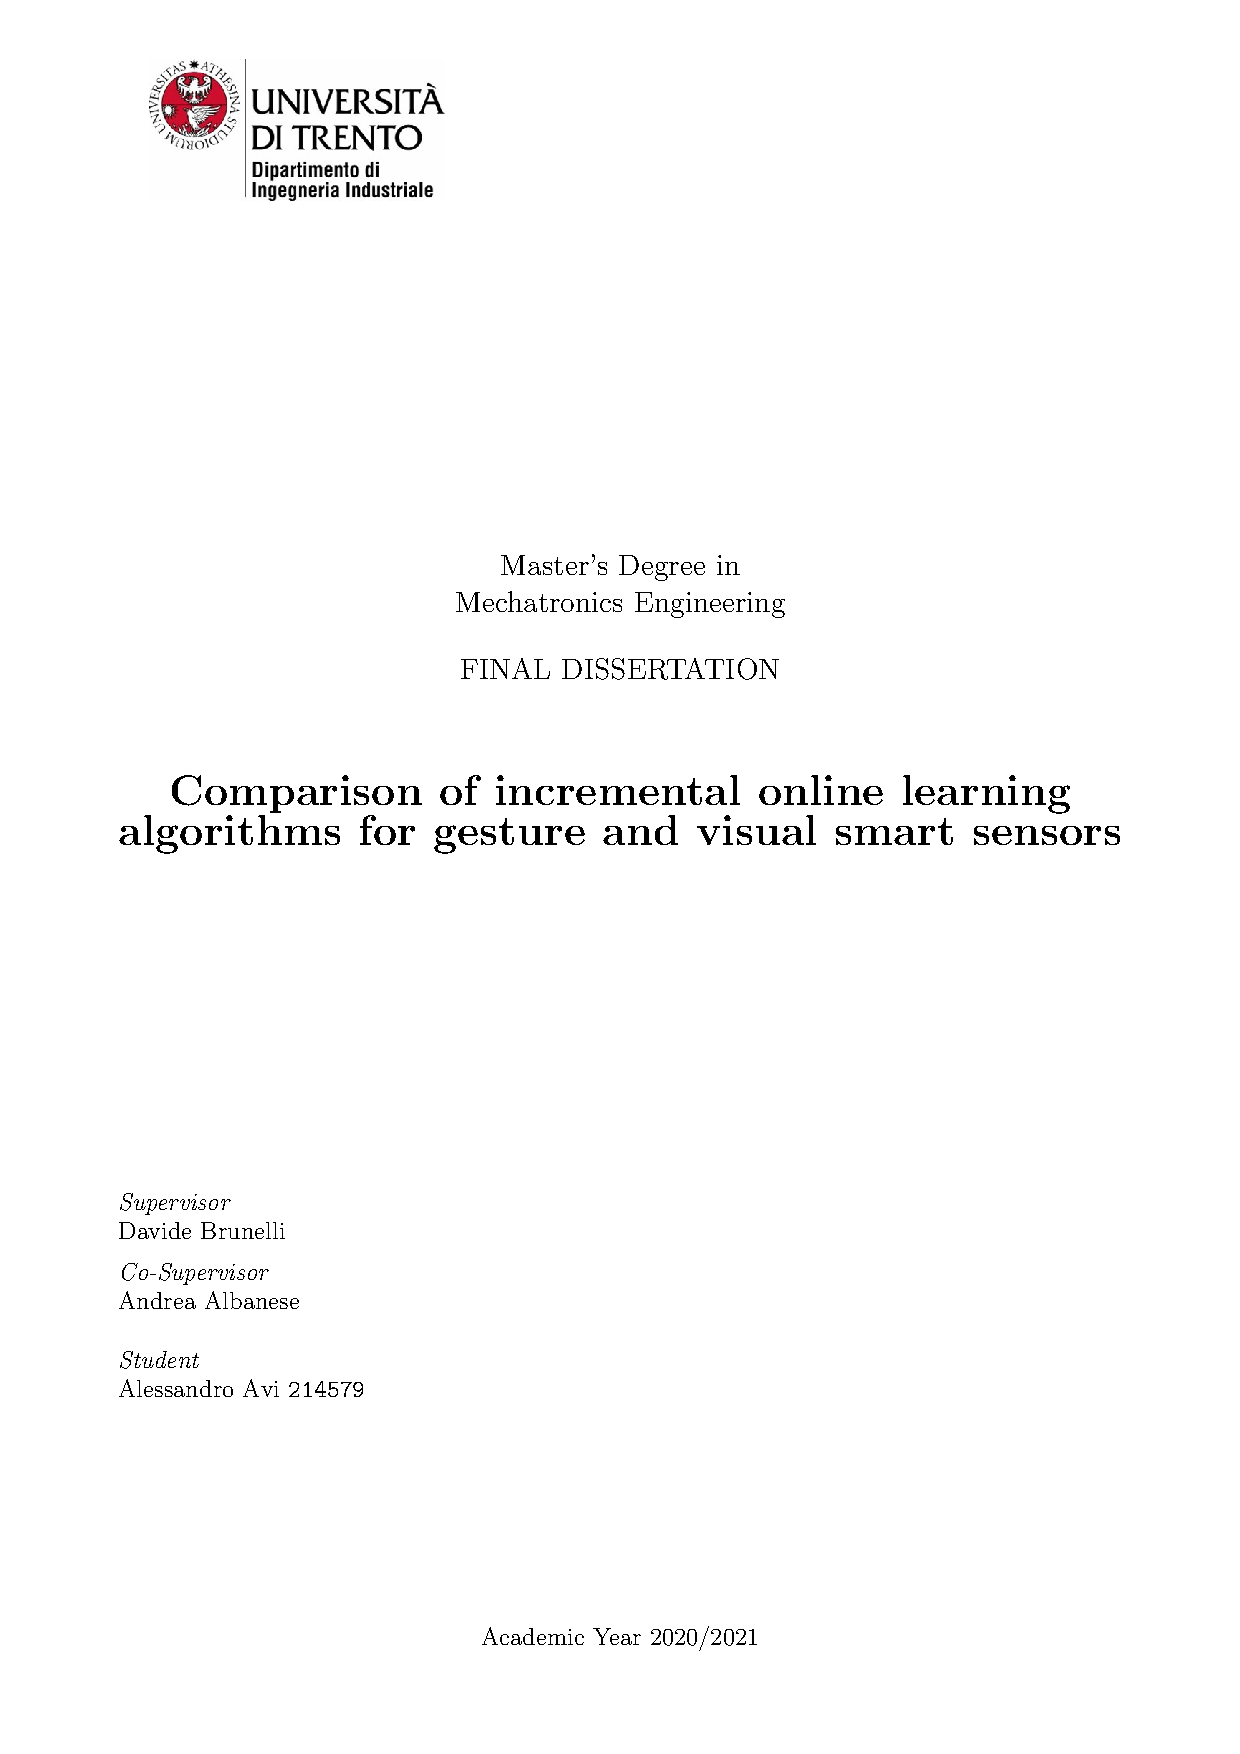
\includepdf[pages=-]{Figures/frontespizio.pdf}
\end{figure}

\afterpage{\blankpage}

\chapter*{}
\vspace*{\fill}
\textit{"Frase"} 
\begin{flushright}
Mario Rossi
\end{flushright}
\vspace*{\fill}

\afterpage{\blankpage}





%\afterpage{\blankpage}
\tableofcontents
%\afterpage{\blankpage}
\listoffigures
\listoftables
\afterpage{\blankpage}



%\mainmatter

\mychapter{0}{Introduction}
\pagenumbering{arabic}

Machine learning (ML) applications on small devices, known as TinyML, is becoming more and more popular. The usage of this type of technology on micro controllers (MCU) is becoming more and more indispensable and helpful in several fields such as industrial applications, agricultural automation, autonomous driving and human-machine interaction. One of the main fields in which TinyML is well suited is Internet of Things (IoT). Here, machine learning is applied on small devices and it can be exploited to revolutionize the basics of IoT networks.\\
The ability of embedded systems to perform high-level and smart data elaboration makes it possible for the IoT pipeline to change from cloud computing to edge computing. This transformation comes with great benefits and additional challenges. 
First of all, the traffic on IoT networks is drastically reduced. In fact, by performing inferences and predictions directly on the edge the raw data gets compressed into smaller sequences that are dense of information, reducing the quantity of data moving in the IoT networks. This allows to diminish the energy consumption dedicated to the entire system as well as the system responsiveness and efficiency. 
Edge computing lowers the traffic in IoT systems but also reduces the computational weight in the cloud servers. This results in reduced times of computation and communication between edge and cloud which, if combined with the ability of the MCU to perform autonomous decision, reduces the latency of real time applications improving the overall experience. 
Moreover, IoT network privacy issues can be addressed by reducing transmitted data, and consequently reducing the possibility to have unwanted interceptions. 
At last the usage of ML on small devices allows to better customize the device, and make the devices better suited for specific jobs. \\
Of course, the application of such a technology comes with a cost, which is the increased complexity and higher amount of vulnerabilities. Thus it is necessary to set up robust systems that are able to ensure the system security (due to the high number of vulnerable nodes), and high performances, no matter the limitation of the device. It is in fact known that the main downsides of embedded systems and small MCUs are their limited hardware, small memories, and low-capacity batteries. Another important aspect concerning TinyML is the training and deployment of the model, which is typically performed on a powerful device and later loaded on the MCU using compression strategies. The main challenge is how the compression of big and well performing models is performed, especially because the model needs to maintain high accuracy with a low memory footprint. The creation of efficient and optimized compression strategies has been one of the main focus of recent research in the TinyML. \\
Another relevant challenge for the application of ML in IoT systems comes directly from the environment in which IoT smart nodes are deployed. Depending on the specific application, it is usually the case that the context in which an IoT device works is not characterized by a static behaviour. Meaning that the phenomenon to be monitored is able to change or evolve over time, thus recorded data can consequently evolve and change its main features. This can make difficult using ML models because they only perform inference and lack the ability to adapt to changing scenarios. It is clear how devices, set up in this way, are vulnerable to the context drift aforementioned. 
By training ML models for a specific context and later deploying them in the real world, it is expected a drop in accuracy which can make the application itself not reliable. It is then obvious how an application of simple ML inference on such environments is not the best solution. To contrast this issue, it is necessary to implement the so called Continual Learning (CL) algorithms. CL is a machine learning approach that allows ML models to perform training in real time and continually keep up-to-date the model weights. The implementation of this method comes with new challenges and limitations which are mainly related to memory management and strategies for the implementation of real time training which also keep in consideration the optimization of resources.
\bigskip

Continual learning methods lead to a real time training based on the data incoming. This allows the model to change and fine tune its weights and structure to better contrast the context drift. 
An additional feature that can be easily added to CL is the ability to recognize never seen classes. This, if paired with the model's ability to extend its structure, allows to create a flexible model that is able to allocate new weights and biases for better predictions.  
An important problem that tackles basic applications of CL is catastrophic forgetting. Catastrophic forgetting is a phenomenon that occurs when model trained in real time overfits new data. This makes the knowledge related to past tasks be replaced by new knowledge, thus forgetting the initial scenario which leads to a reduction of the model performances over time. This aspect can be reduced by applying preventive mechanism inside the back propagation that control the parameters update. \\
The implementation of CL in industrial applications is not a new topic in the research world, but its implementation on tiny devices is just started to become more and more popular. One common application is CL in industrial scenarios, mainly for monitoring purposes on heavy machines.
The main contributions of this study concern the application of CL in two different applications. The objective is to understand if CL is a feasible solution for TinyML and if its use is actually effective for the generation of autonomous and self adapting models. In this study, a light framework that is easy to connect to a pre trained classification model was developed. The system substitutes the last layer and continually performs updates on weights and biases, and also extends its shape for flexible adaptation to new classes. The system is able to use different state-of-the-art strategies that are tested and compared in two experiments with the aim of understanding if it is possible to: i) maintain or improve the accuracy of the model; ii)contrast catastrophic forgetting; iii) digest and learn classes of never seen data. Both experiments concern the application of ML for the classification of data coming from different sensors. \\
The first application regards the analysis of accelerometer data. In this experiment the user holds the accelerometer sensor in its hand and records a time series of accelerations while drawing letters in the air. The idea is to apply ML to classify the data and recognize the letters written. The model created is initially trained for the recognition of the pattern that characterize the five vowels. Later CL is applied to the experiment and the model is exposed to new data representing three new consonants. The aim of the experiment is to let the ML model learn new patterns by performing a real time training.
The experiment can be considered a simplification of a real world applications, but it is a clear example of how a CL model can behave in these scenarios. This application can be extended in a real-life scenario such as the monitoring of vibration patterns of heavy industrial machinery. \\
The second application concerns the experimentation of CL on a CNN model applied on an OpenMV camera for the visual recognition of digits from the MNIST dataset. The idea consists of initially train the model to recognize only the digits from 0 to 5 and later use the CL framework developed for applying a real time training on the remaining digits. This second experiment can be extended to applications where a camera is used for a visual control of defects on products in a production pipeline.  \\
The work carried out in this study shows that the application of CL on tiny devices is possible. Even though the CL strategies are applied only on the last layer the results are satisfying and in both examples all the classes were correctly digested by the model. These tests show that a model equipped with a CL system is able to expand its knowledge and learn more classes, specifically 3 for the letters example and 4 for the digits example. The devices are able to maintain a reasonable accuracy at the end of the trainings that drop from the original frozen model accuracy by only 10\%. 
The study performed is a good example that shows the capabilities of these tiny devices. It proves that machine learning applied on MCUs is a technology that has a huge potential and deserves more attention. CL can lead to smarter, more efficient, better performing systems in the IoT field and in industrial applications.
\bigskip

UNA VOLTA DEFINITA UNA STRUTTURA CHIARA E PRECISA PER IL RESTO DELLA TESI SCRIVERE 4/5 RIGHE PER OGNI CAPITOLO/SEZIONE
% struttura tesi/Come organizzata. faccio spiegazione di contenuto su ogni capitolo (4/5 righe a capitolo). 


\chapter{Related Works}

In this chapter some information about the application of machine learning on tiny devices are given. Then a brief introduction to continual learnin is done with a following explanation of the most relevant state-of-the-art studies regarding continual learning in TinyML world. 

\section{Machine learning in general}

\section{Cloud vs edge inference}


\section{Machine Learning on MCU}
% applicazione ml su mcu, risorse limitate, molto importante power comsumption, design del mcu, paralre di possibili applicazioni, paraldre del fatto che si fa solo inference
% parlare del rpuning, binarization, compression del meodello, state of teh art compression MCUNET


TinyML is a fast growing research area that aims at applying ML on limited devices like micro controllers. This technology has found a rapid grow in the last years especially thanks to the potential demonstrated by its application in several fields like industrial application, agricultural automation, human-computer interactions, autonomous driving. The use of TinyML in all these fields allows to introduce the concept of edge computing, where computations are brought closer to the origin of the data, to devices that up until now have been used only as collector and transmitters of data. Edge computing bring to lots of advantages like low-latency , better privacy, security and reliability to the network end-user. It allows to move the computations from the cloud to the device itself, which brings to higher throughput and improved responsiveness in applications. Speaking about responsiveness, which is a huge deal for real time applications, edge computing permits to decrease the network traffic. This feature comes from the fact that the use of machine learning directly on the device allows to lift a big portion of computation weight given to the central server, thus reducing the amount of data that has to be exchanged on the network, which is also compressed in size and dense in information. \\
One of the main fields in which TinyML is particularly fit and can be exploited with all its potential is for sure the world of IoT. Here the application of edge computing brings to lots of advantages already described before. Of course the implementation of such systems comes with a cost, which in this case is related to the increased complexity on which the MCU works and its limited resources. Machine learning is a field of computer science that is known to be energy and resource demanding. Using such a technology on these tiny devices is a real challenge which already has seen interesting applications and improvements in the research world. The main characteristic of MCU is for sure their limited dimensions and power consumption. This is usually a nice feature that allows to develop small systems that can live for very long period of times in harsh environments without the need of maintenance. 
Lot of focus has also given to the implementation of energy harvesting systems that, not only use very low quantities of energy but also are able to extract energy from the environment in which they live. Limited dimensions has also drawbacks, which are limited memories and limited computational power, all features that do not really match with the application of machine learning. 
In the last decade (??) the research around TinyML revolved around the implementation of efficient framework from both point of view of memory use and power consumption. Some well known systems for deployment of ML models on tiny devices developed by big companies are Tensorflow Lite \ref{}, STM32 CUBE AI \ref{}, PyTorch mobile \ref{}. All these frameworks are used for training a model on a powerful system and later load a compressed version of the model on the MCU. The main concerns is the compression of the model in such a way that it doesn't drop in accuracy even with reduced weights or quatnized values. The second aspect that concerns the use of these tools is the inferenfce performed on the device. Being that procedure computationally heavy it's necessary to be able to optimize the computations. Some research studies focused soecifically on this.





The main challenge of TinyML is for sure the successful application of ML on such resource constrained systems. These are in fact designed to be deployed in difficult to reach places and for running for very long times. This implies that the devices should be battery power or equipped with energy harvesting hardware and their power consumption should be limited and optimized. Other limitations concern the limited computational power, which is directly connected to the CPU frequency and the battery management and the available memory. The latter is a very important topic for TinyML. It's in fact known that the application of ML on any type of device requires the usage of great amounts of memory, it's then a big challenge to be able to deploy these systems with very limited memories.\\
The application of ML on MCUs, mobile devices or in general on the edge of IoT systems it's a great advantage that can bring to some improvmenets. The key advantages are:
\begin{itemize}
\item privacy: by having the data directly processed on the node there is no change of violating the privacy policies since the possibility of interception is totally nulled
\item latency: by elaborating data directly on the edge the work load of processing that should be performed by the cloud is limited and so is the transmission of the data itself. This brings to limited time delays and allows the device to perform decisions in real time, improving the performances of real time applications.
\item energy efficiency: the transmission of huge quantities of data from the edge to the cloud takes a big portion of the energy consumption of an IoT system. Even if the application of NN is energy intensive it is an order of magnitude less, thus an improvement.
\end{itemize}


\section{Continual-on line learning}
% spiegare cosa è ctastrophic forgetting, come mai serve, cosa va a risolvere, quali sono i problemi che iontroduce, 
% parlare di cinme CL è trattato nella research, paralkre dlle tipologie di algoritmi, supervised training, frameworks gia sviluppatim metodi di valutazione?

Until recent times the application of ML on MCUs has always been focused on the creation of intelligent small system that maintain good performance with reasonable consumption, limited time of inference and long lifetimes. A major negative aspect of the TinyML solutions is their focus on the inference of streams of data. Which almost always requires the usage of powerful machines for the training of NN models that are later deployed on the MCU. This results in the creation of a static network which is not able to adapt to the data and adjust to different scenarios. The solution to this problem is the creation of a Continual Learning system. \\
CL systems are a variation of the tipical pipeline of ML. The main focus of CL systems is to be able to continuously update the model in order to adapt its structure and parameters to overcome context drift, be able to recognize appearance of new patterns and to avoid catastrophic forgetting. The latter is a problem that is directly introduced by the nature of the paradigm itself. By having a model that is continuously updated with a feedback loop that is directly dependent on the current erross i'ts clear how it's immediate to update the model in such a way that the old tasks are forgetten for the sake of learning the new ones. This could be seen also as a over fitting of the model on the new tasks and if oc course to be avoided. Different algorithms have different ways for contrasting this phenomenon. \\
In todays literature several CL algoprithms and strategies have been already proposed. A well organized summary is proposed in \cite{lesort2020continual}, where the most relevant methods are briefly classified in 4 categories, originally proposed by \autocite{maltoni2019continuous}.
\begin{itemize}
\item Architectural: these algorithms are based on the usage of particular types of structures and architectures. Some common methods are weight-freezing, layer activation or dual-memories-models that try to imitate logn term memory and short term memory.
\item Regularization: this group contains all those approaches that base their ability to retain past memories on the application of particular loss functions. In these loss functions usually a term is added with the aim of performing a feedback that considers both the old knowledge and tries to learn the new data.
\item Rehearsal strategies: in these strategies past informations are periodically revisited by the model. This is done for strengthening the old knowledge and connections. Notice that this methods is not well suited for application on MCUs mainly because of the restricted memories. 
\item Generative Replay: this methods implement similar strategies of the rehearsal. This time the data that is repeated in the models is not actually old data saved in the memory but it's actually data artificially generate by the model itself. 
\end{itemize} 

The type of strategies that better suits an application on MCU are for sure the regularization methods and the architectural methods. Both these groups require little to no extra computation with respect to a simple ML application, thus their strength is intrinsic in the update rules adopted. Some of the most important methods from the state of the art are, LWF, PNN, CWR, EWC, SI. 



\section{Pruning and quantization}





\chapter{Hardware} 
\label{chap:hardware}
In this chapter the hardware used to carry out the experiments is described. The application of ML on MCU does not require a specific type of device or specific peripherals. The devices should be equipped with memories (RAM and flash) big enough for containing the pre-trained model and for performing inference.  Then the device should be equipped with a CPU capable of sustaining ML computations, even if optimized, in short periods of time. In today's market lots of off the shelf devices with ML capabilities are already available. The most common are from Arduino, Raspberry or STM32, which only feature devices powerful enough for performing inference. For this study it has been decided to use two MCUs for the two applications, where both devices are based on STM32 components. The first experiment uses an STM32 Nucleo F401-RE, a well performing and easy to use development board. The second application uses an OpenMV camera, a device equipped with a camera sensor that uses an STM32 H7 MCU and is programmable in MicroPython. Figure \ref{hardware_all} shows both devices, on the left the Nucleo F401-RE, on the left the OpenMV camera.
%
\begin{figure}[h!]
    \centering
    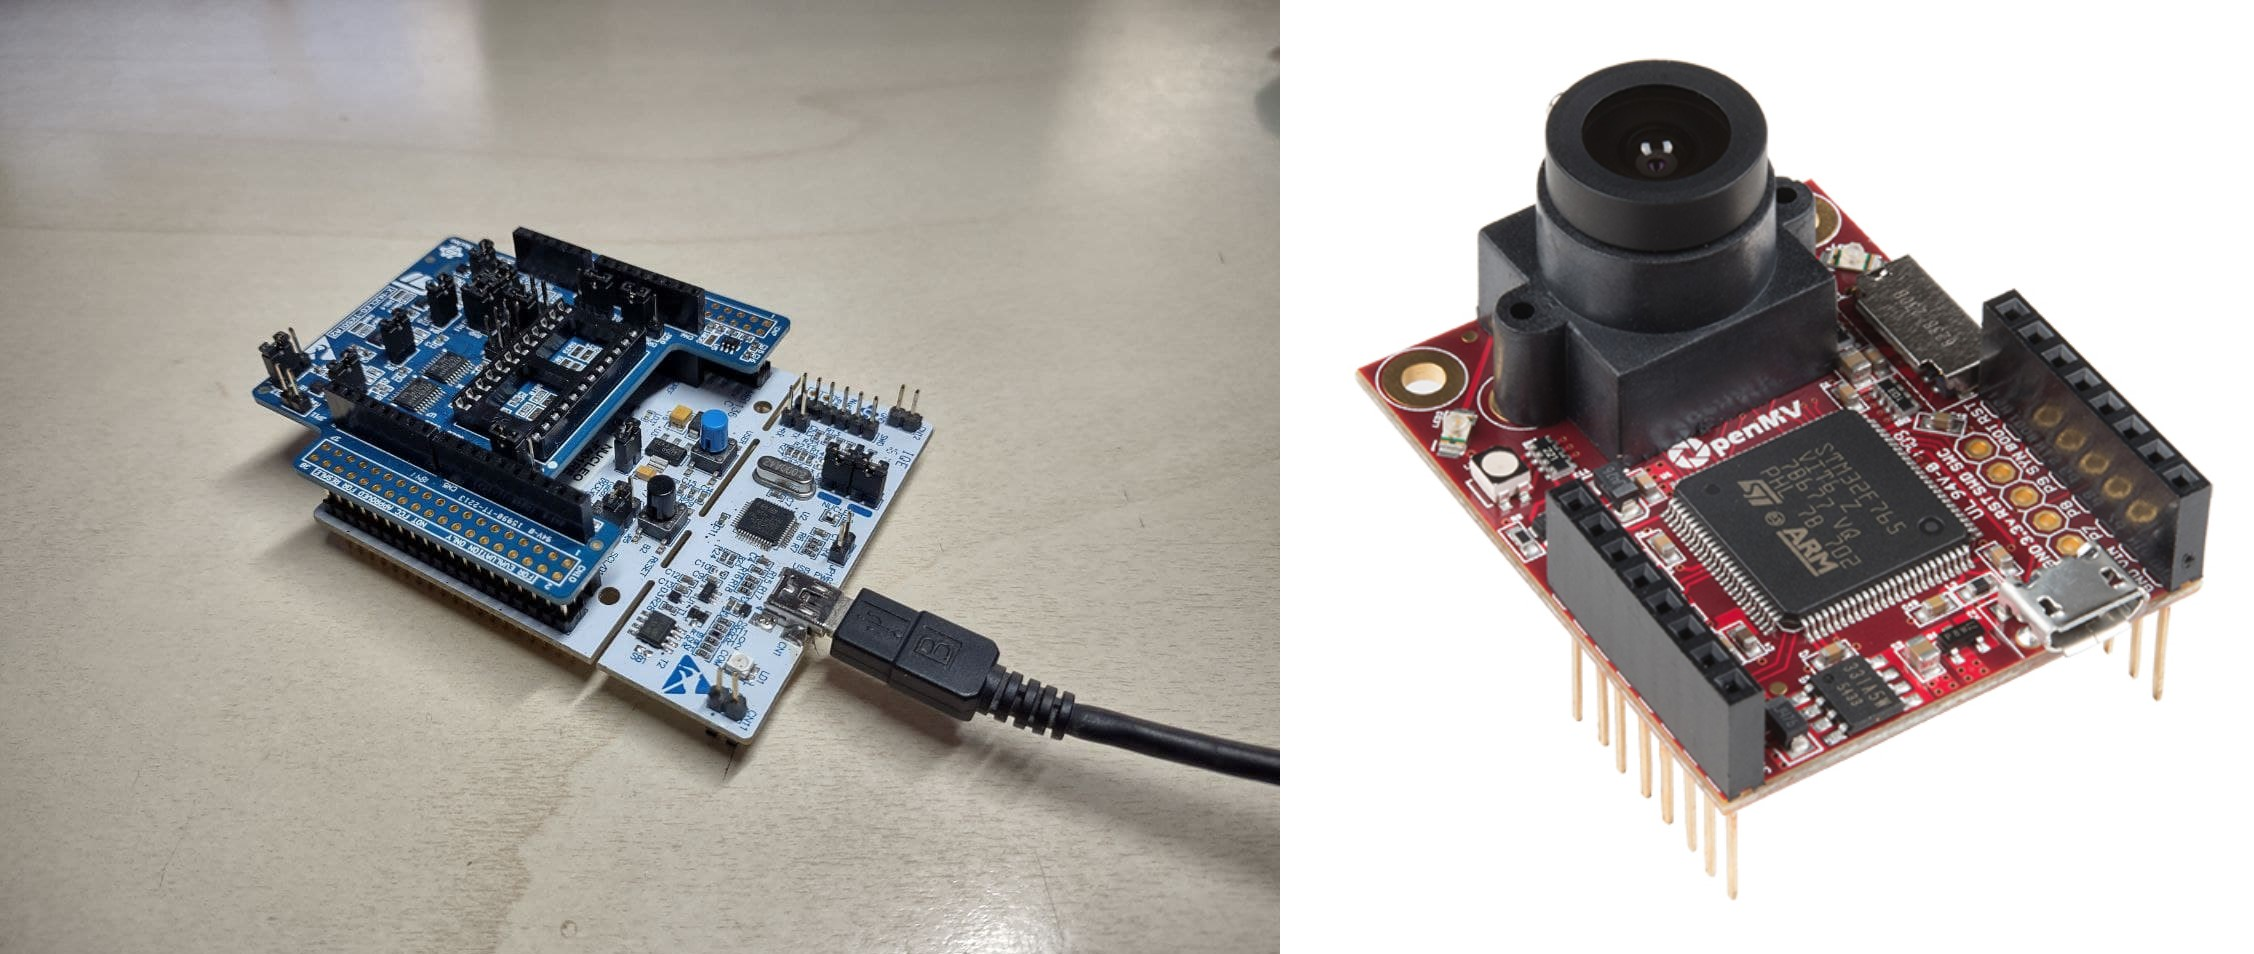
\includegraphics[width=0.7\textwidth]{Figures/Chapter2/hardware.jpg} 
    \caption{PLACEHOLDER}
    \label{fig:hardware_all}    
\end{figure}
%

\section{Gesture recognition hardware}
The experiment is carried out with a Nucleo STM32 F401-RE. This type of device is an easy to use development board that can be programmed in C or C++. It fully supports the extension pack STM-CUBE-AI \autocite{stm_cube_ai} developed by STM used for loading, compressing and performing inference in real time. \\
The main features of the development board are summaryzed in Table \ref{tab:specifications_openmv}.

INSERIRE TABELLA CON DATAI DEL NUCLEO

The application for gesture recognition is based on the analysis of accelerometer data recorded while drawing letters in the air. To acquire that kind of data the Nucelo needs to be equipped with an accelerometer sensor. For doing that it has been decided to use a Nucelo shield, also developed by STM called IKS01A2 \autocite{shield_web_page}, which can be easily mounted on the Nucleo board simply by aligning the pins. The shield is equipped with a 3D accelerometer, a pressure sensor and a capacitive digital relative humidity and temperature sensor. The shield communicates with the Nucleo through I2C protocol and its use is completely supported by STM libraries, which make its use simple and fast. Figure \ref{hardware_stm} shows the two devices separately on the left and mounted on the right.
%
\begin{figure}[h!]
    \centering
    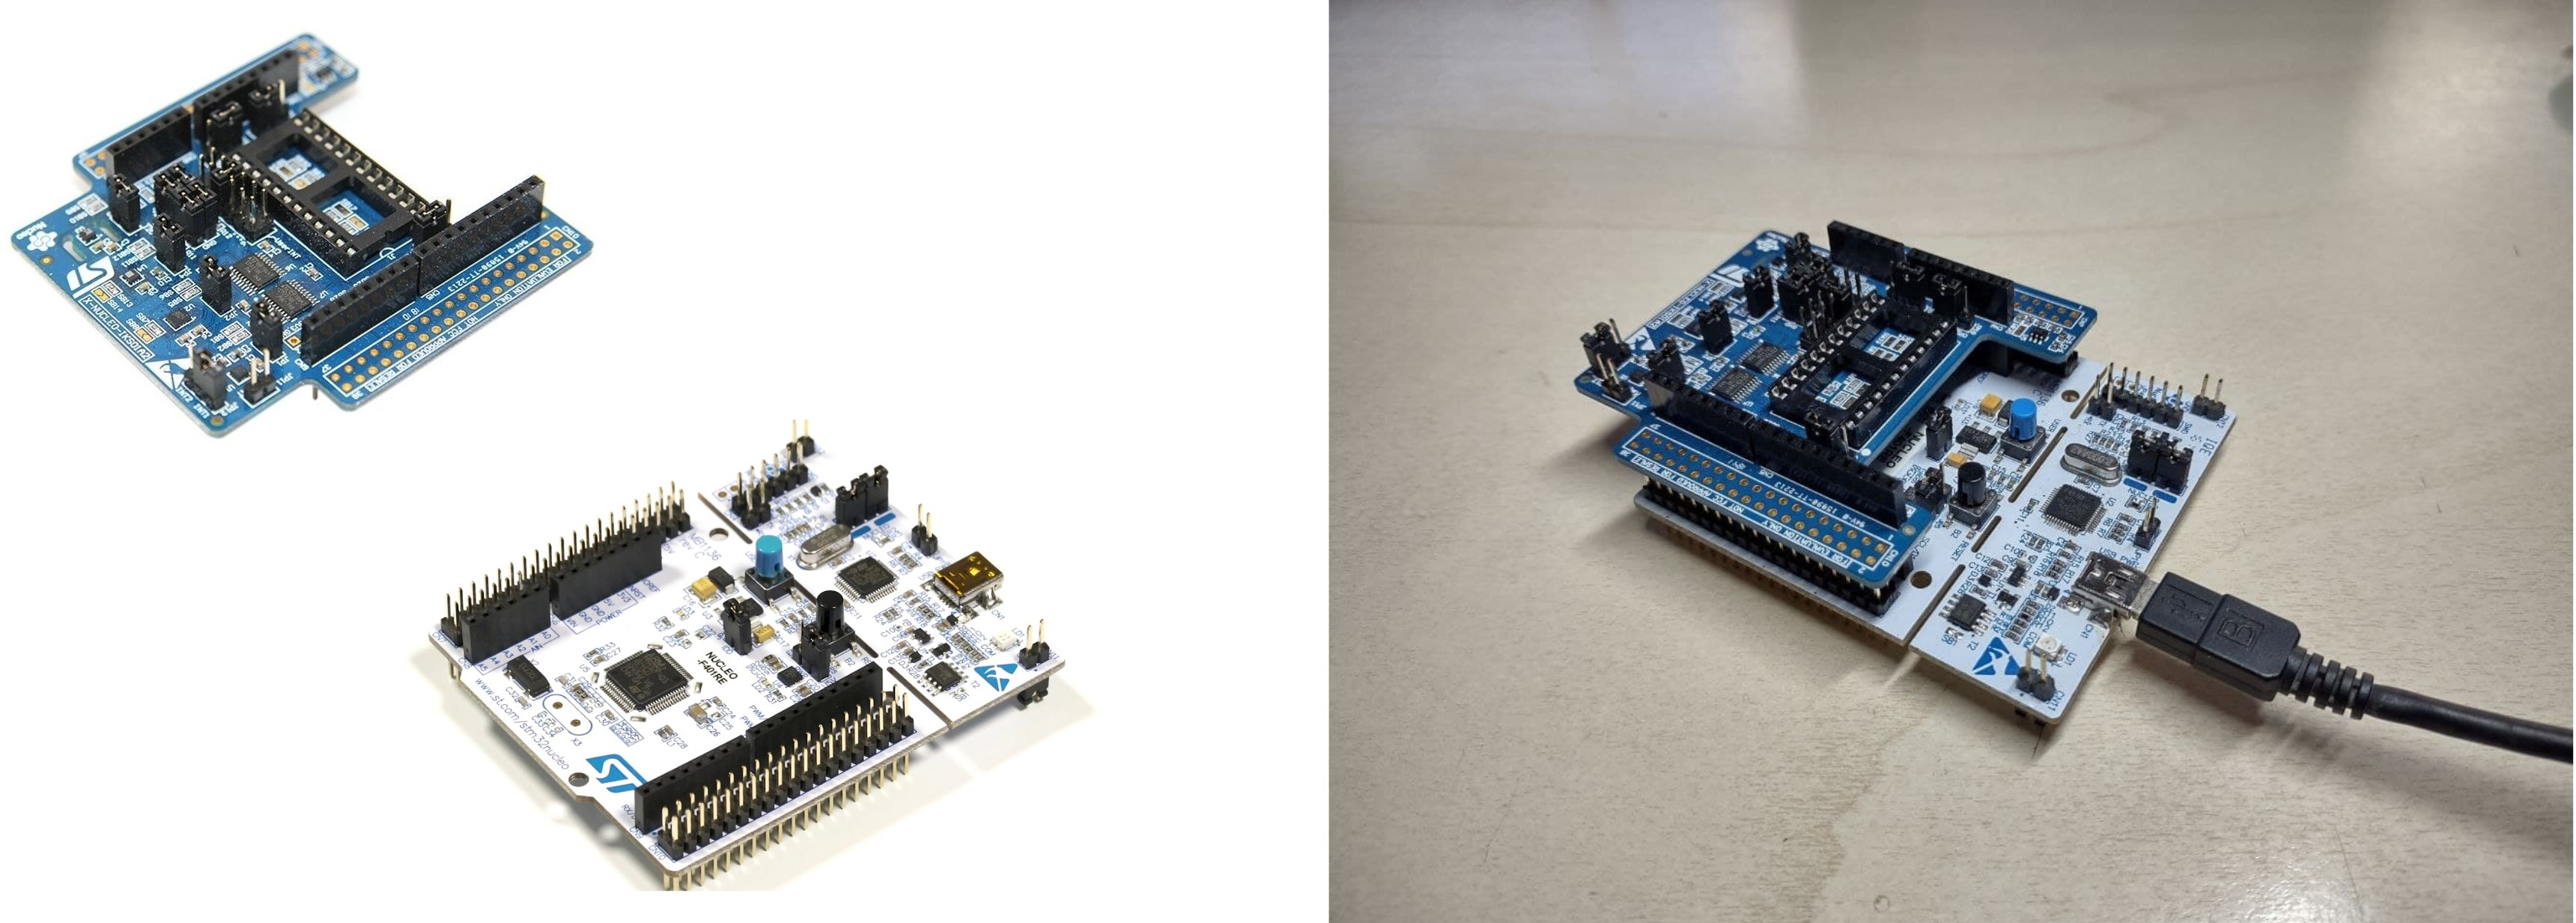
\includegraphics[width=0.7\textwidth]{Figures/Chapter2/hardware_stm.jpg} 
    \caption{PLACEHOLDER}
    \label{fig:hardware_stm}    
\end{figure}
%
\subsection{STM-CUBE-AI}

\section{Image classification hardware}
For the second experiment an OpenMV 	\ref{openmv_web_page} camera is used. This device is a small board equipped with an STM H7 MCU and a camera sensor with interchangeable lens. The board mounts also some GPIO pins thanks to which is possible to use interrupts, I2C, UART, SPI an many other peripherals. The OpenMV camera is a project developed from a kickstarter which got increasing attention and became to be a well performing piece of hardware. The device is thought to be deployed specifically in computer vision scenarios, with the possibility to drive external motors, robots, drones or use machine learning. It has been decided to use this hardware because of its relatively low cost, its high computational power, ease of use thanks to MicroPython and the support and continuous updates that are developed. Additionally the camera is supported also by external hardware modules such as Wi-fi modules, interhcangable lens (IR, fisheye, different focal length), screen shield, CAN shield.\\
Table \ref{tab:specifications_openmv} summarizes the specifications of the device.

\begin{table}[]
\begin{tabular}{|l|c|}
\hline
Processor           & \begin{tabular}[c]{@{}c@{}}ARM 32-bit Cortex-M7 CPU\\ w/ Double Precision FPU 480 MHz (1027 DMIPS)\end{tabular}                               \\ \hline
Memory              & \begin{tabular}[c]{@{}c@{}}SDRAM: 32 MBs\\ SRAM: 1 MB\\ Flash: ext 32 MB, int 2 MB\\ Expandable with SD cart\end{tabular}                     \\ \hline
Resolution          & \begin{tabular}[c]{@{}c@{}}Grayscale: 640x480 max\\ RGB565: 320x240 max\\ Grayscale JPEG: 640x640 max\\ RGB565 JPEG: 640x480 max\end{tabular} \\ \hline
Phisical attributes & \begin{tabular}[c]{@{}c@{}}Weight: 19g\\ Length, Width, Height: 45x36x30 mm\end{tabular}                                                      \\ \hline
Lens                & \begin{tabular}[c]{@{}c@{}}Focal length: 2.8mm\\ Aperture: F2.0\\ Format: 1/3"\\ HFOV: 70.8°, VFOV:55.6°\end{tabular}                         \\ \hline
Peripherals         & \begin{tabular}[c]{@{}c@{}}GPIOs, interrupts, SPI, UART, I2C, DAC/ADC,\\ PWM, LEDs, removable camera module\end{tabular}                      \\ \hline
\end{tabular}
\label{tab:specifications_openmv}
\caption{OpenMV H7+ specifications}
\end{table}

To be able to use correctly the device for the application of CL on digits recognition a 3D printed support has been created. Since the continual training is carried out by pointing the camera to the computer screen while frames of the MNIST digits are shown it was necessary to maintain the camera in a still position. A small 3D printed tripod found on Thingiverse \autocite{tripod_link} has been edited to be able to support the camera with minimal modifications. The $stl$ file can be found in the repository of this project \autocite{github_repo}. Figure\ref{fig:hardware_openmv} shows the OpenMV mounted on the 3D printed tripod while pointing t the computer screen during a CL session.
%
\begin{figure}[h!]
    \centering
    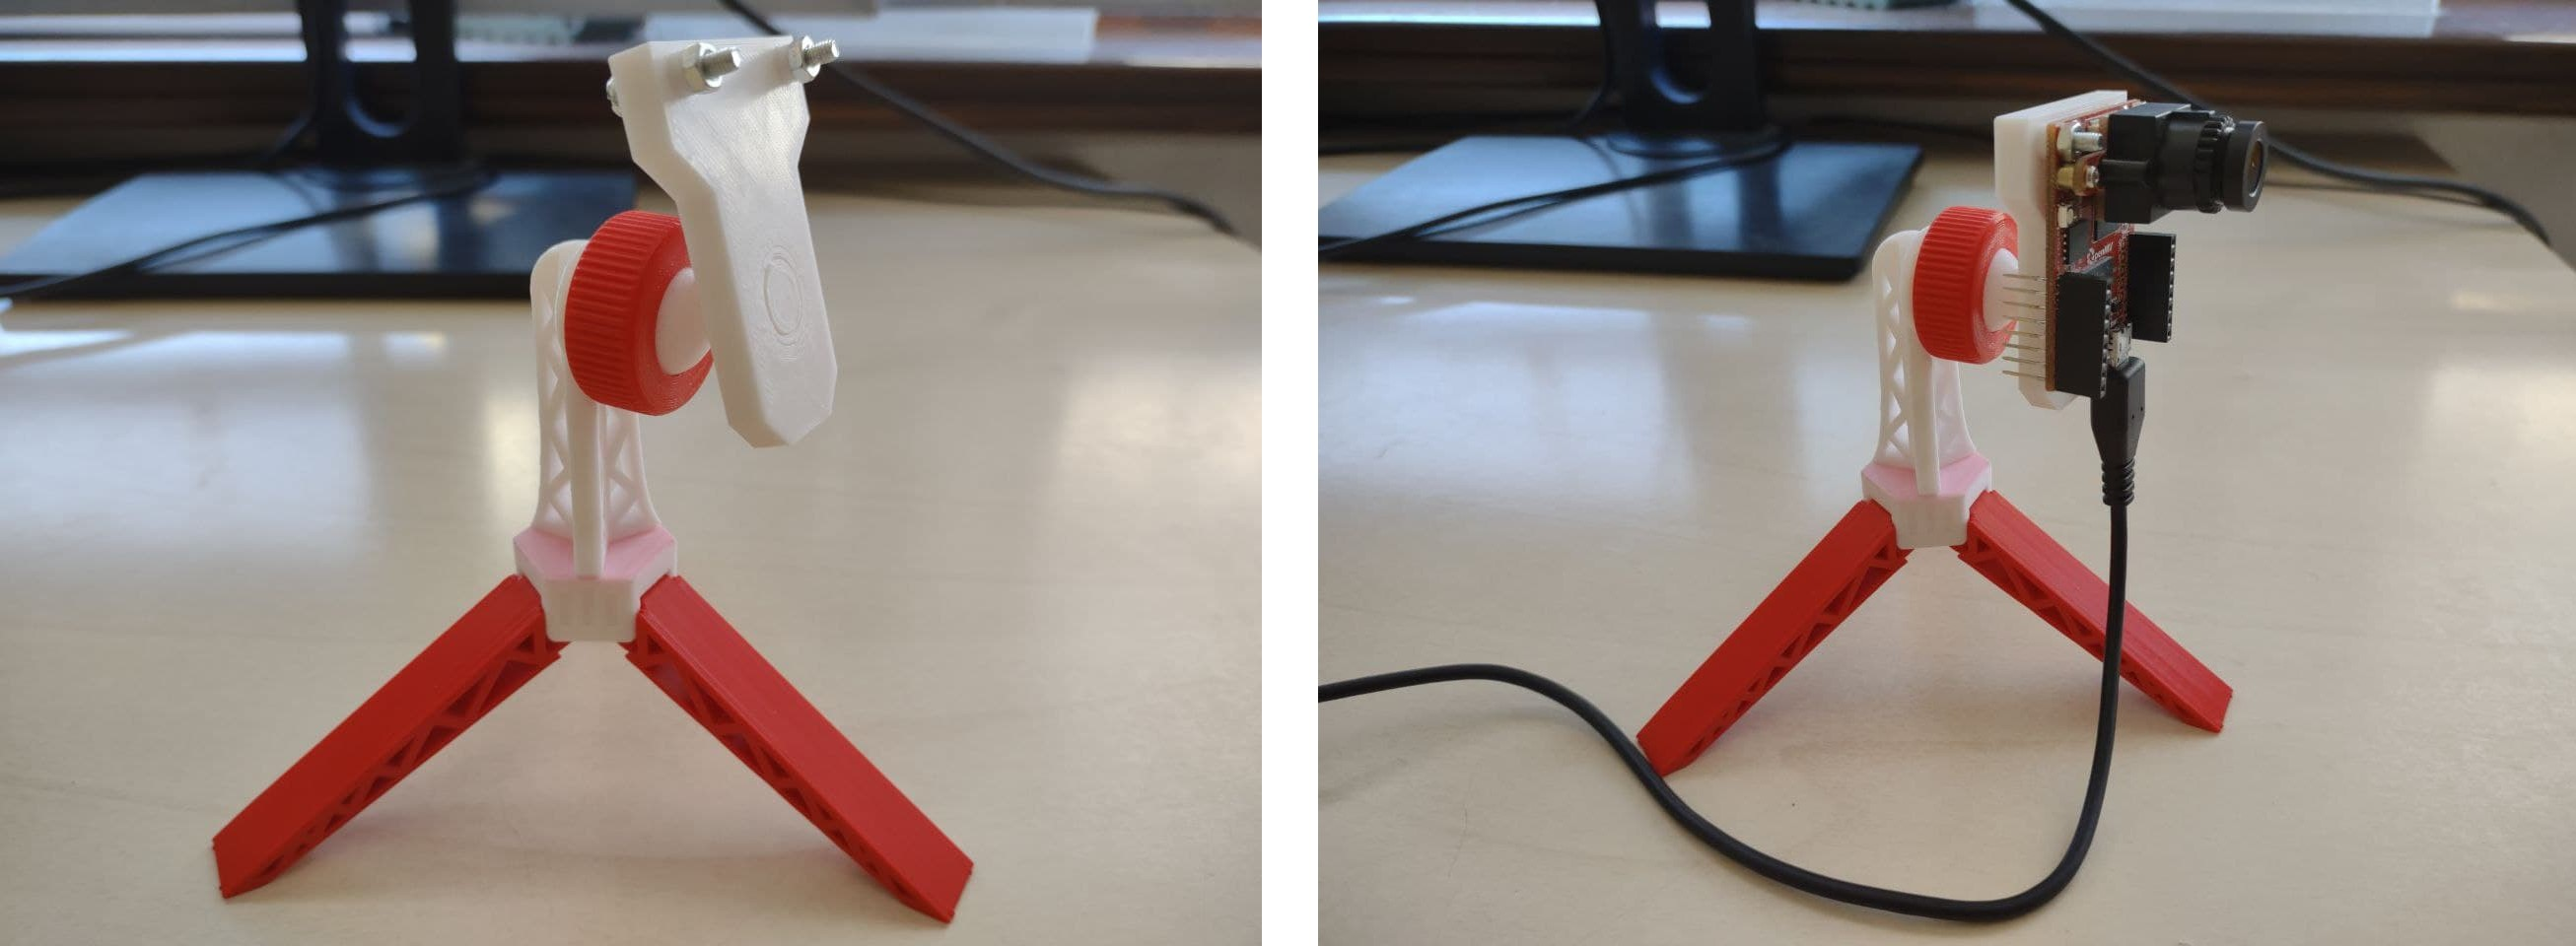
\includegraphics[width=0.7\textwidth]{Figures/Chapter2/hardware_openmv.jpg} 
    \caption{PLACEHOLDER}
    \label{fig:hardware_openmv}    
\end{figure}
%


\chapter{System implementation}
% introduzione la machine learning
% spiegare il funzionamento base, nodi, activation function, layers, 
% CNN, NN fully connected, a cosa servono, quali sono gli obbiettivi specifici
% back propagation, sgd, l rate, batch size
% pruning, quantization

Machine learning is a branch of artificial intelligence (AI) and computer science that focuses on the usage of algorithms and huge quantities of data to generate models that are able to perform regression of grey mox models. 

\section{Basic pipeline of the CL system developed}
\label{basic_system}
% spiegare idea di base del CL in questo caso, training fatto in real time
% spiegare come si ottiene la back propagation, far vedere formule, applicate a softmax
% spiegare il sistema fatto a frozen model + OL layer
% spiegare nel dettaglio i metodi implementati + grafici a blocchi che mostrano come va
Continual learning is the application of real time training on a model with the aim of generating self adjusting systems that are able to learn from the incoming data and modify their properties to adapt changes. As well explianed before continual learning in today's technology finds its best application in IoT edge nodes, where ML is applied on small devices to distribute the computation weight over a large number of devices and reduce the traffic over the network. The main advantage brought by CL or OL is that models are then able to autonomosly update their parameters, ability that improves the easo of use of these devices which can then be ddeployed in environemnt with minimal effort for maintainance. \\
In order to apply such a technology on embedded devices is necessary to develop or use the avilabel software and hardware on the market. For this study the hardware uses are just commercially available MCU that are specifically developed for supporting big quantities of computations. The software used by the microcontrollers on the other hand is only partially developed. In both applications it has been possible to use already developed tools specifically built for inference, which is just one of the steps required for a continual learning application. \\
In this study the main idea was to develop something similar to paper TinyOL. The idea is to attach the OL system to the last layer of the pre trained model in order to enhance just the classification aspect of the ML model. The base functions required by the system are basically two: be able to update the weights of the classification layer each time the model shows an error in the prediction array and be able to enlarge the size of the last layer at will, specifically when new classes are detected that should require a new label. The applications seen here are supervised machine learning trainings. This means that at every training step the griund truth label is known and is provided to the algorithm, which will then use these info to compute the error and back propagate this for updating the layer. In fact the feature that allows the model to recognize new classes is performed simply by checking if the label recieved is inside the pool of already known classes. \\
The basic idea of continual learning consists in being able to continually refresh and update the weights and biases of the layer or layers of interest. This is performed as in standard trainings by computing the error performed by the inference and by propagating its error back in the weights themselves. In orrder to do this it's necessary to know the basic structire of the model wich gives informatiosn about the math used by the nodes. If the entire path of computation from the weight of interest to the final prediction is known then it's possible to back propagate the error to the parameter. In this specific study the idea has always been to use CL in classification problems. By havinsuch a specifica field of application it's possil e to simply the CL ide to a restricted group of models. Since the problems regard only classification and this specifica application want sto update only the lsat layer the problem becomes a simple study of the back propagation over softmx layers and nodes. Let's consider a simple model composed of few layer, and asume that the last layer brings 100 nodes of the hidden layer 2 to just 5 nodes with softmax application function. It's then possible to comnsider everythin that happens before the softmax layer a grey box that simply gives us 100 output values. The basic formulas used ina  softmax layer are the following:

\begin{equation}
z_i = \sum_i w_{ij} x_j + b_i\\ 
y_i = softmax(z_i) = \frac{e^{z_j}}{\sum_j=1^k e^{z_j}}\\
\text{where  i = 1, 2, ..., k     j = 1, 2, ..., n}\\
\text{where  k = number of classes known by the model}\\
\text{where  n = number of outputs from the frozen model}\\
\end{equation}

Where equation x is the formula that describes the the basic computation of a node of a ML layer, equation 2 is the softmax function directly applied on the ouput computed by the node.
The complete computation for the output of the OL layer then becomes:
\begin{equation}
	y_i =  softmax(z_i) = \frac{e^{\sum_j=1^n w_{ij} x_j+b_i}}{\sum_j=1^k  e^{\sum_j=1^n w_{ij} x_j+b_i}}
\end{equation}

Once the prediction is computed with the softmax function applied on the output of the nodes, it is possible to use the loss function and compute the error. In common machine learning application the list of possible loss fuicntion that can be used is long and the different costs can be selected for different reasons and applications. In this case it has been decided to use a $categorical$ $cross$ $entropy$, which has the following definition:

\begin{align}
	cost = - \frac{1}{n} \sum_k [ y ln(y_i)+(1-t_i)ln(1-y_i) ]
\end{align}

Where $n$ is the total number of training data, $y_i$ is the output obtained from the softmax function, $t_i$ is the true label. \\
At this point the entire path of computations from the output of the frozen model to the error committed by the prediction is known. This allows for the computation of the derivatives iof such error which are necessary for the back propagation, where the weights and biases of previous layers are updated with a proportional dependancy on the derivativo of the error with respect to every single weight. The computations performed for the final update rule are the following:


\begin{align}
	\text{Given that the error E is computed as: } E = cross(y_i) = cross(soft(z_i))  \\
	\frac{\partial  E}{\partial  w_{ij}} & = \frac{\partial  E}{\partial  S_i} \cdot \frac{\partial  S_i}{\partial  z_i} \cdot 	\frac{\partial  z_i}{\partial  w_{ij}}\\
	\frac{\partial  z_i}{\partial  w_{ij}} & = X_j \\
	\frac{\partial  S_i}{\partial  z_i} & = \frac{}{} = \frac{e^{z_i}}{(\sum e^{z_i})^2} - \frac{(e^{z_i})^2}{(\sum e^{z_i})^2} = softmax(z_i) - (softmax(z_i))^2 = softmax(z_i) - (1-softmax(z_i))\\
\end{align}

Then it's immediate to apply this on the weifht in order to apply an actual training step. The final formula that defines the back proapgation on weights and biases of a softmax layer with the usage of a categorical cross entrioyp loss function is:

\begin{equation}
w = w- l rate
\end{equation}

This is the rule to be followd for the application a basic training step in real time. This is also the same idea explored by TinyOL, which simply applies this rule to an autoencoder model for the recognition of patterns. \\


\section{Algorithms implemented}
In this study not only the basic training strategy has been implemented and tested but also other regularization approaches have been used. As explained in the related work section regularization approaches are strategies that exploit the addition of a loss term to the update. Thanks to this it's possible to have some sort of control over the weight update. In today's research the most efficient and common strategies for CL are Elastic Weight Consolidation (EWC), Synaptic Intelligence (SI), Learn Without Forgetting (LWF) \autocite{li2017learning} and in a recent paper also Copy Weight with Reinit (CWR) \autocite{lomonaco2017core50}, Copy Weight with Reinit+ (CWR+) \autocite{maltoni2019continuous} and AR1 \autocite{maltoni2019continuous} have been presented. In this study it has been considered opportune to implement and compare the simpler ones which are LWF and CWR, together with the basic TinyOL and a small variations of them. \\
In the applications for this study all methods are applied in the same OL general block system, which simply is attached to a pre trained model, called frozen model. The frozen model is treated as a grey box which simply performs feature extraction on the input array and provides the last layer with useful elaborated data. The OL training is then applied on the weights of the classification layer following the update rule imposed by the algorithm of choice.

\subsubsection{TinyOL}

The TinyOL method applied on MCU has been initially implemented in paper \autocite{ren2021tinyol}. Its implementation is quite easy since it consists in just some for loops applied correctly on the weights and biases. As explained before, this method uses the basic rule of the training step which consists of propagating the error committed at inference to the weight of interest by using SGD. Keep in mind that the activation function of the last layer is Softmax and the loss function is always Categorical Cross Entropy. This said the weights update rule for this algorithm are:
%
\[ \mathcal{L}_{cross}(y_i, t_i)= - \sum_i t_i log(y_i) + (1-t_i)\cdot log(1-y_i)  \]
\[    w_{i,j} = w_{i,j} - \alpha (y_i - t_i) \cdot x_i \]
\[    b_i = b_i - \alpha (y_i - t_i) \]
\[    \text{where i=0,1..,n  and  j=0,1,..,m} \]
%
Where $y_i$ is the prediction obtained from the OL layer, $t_i$ is the true label, $\alpha$ is the learning rate (tuned by the user), $w_{i,j}$ are the weights of the OL layer, $b_i$ are the biases of the OL layer, $n$ is the max amount of classes known by the OL system and $m$ is the height of the last layer of the frozen model. Note that in this entire study the number $n$ can change dynamically since the maximum amount of possible classes is not known a priori, or at least it ism not known in a real life scenario. \\
Also a variation of this method has been implemented. The variation takes into consideration the possibility to use batches of data for computing the back propagation and not simply the last sample received. The idea for implementing such a variation came thanks to the article \autocite{batch_size_medium}, where the author explores the impact that batch size has on the training dynamics. The base idea of the variation is that by using a batch of samples bigger than 1 the back propagation computed should not relay on just the last sample but on the average computed on the group. This should help the model to be less vulnerable to noisy data and outliers. In order to apply the algorithm with this variation it's necessary to store the data generated from the previous samples. This requires the allocation of double the amount of memory required for the standard version, which is done with the creation of the matrix W and B. In order to reduce the amount of computation at each training step at first the inference is performed, after this the back propagation for each single weight and bias is computed and its value is added inside the matrices W and B. When the batch finishes the average on each weight and bias is computed and applied on the actual parameter that was kept constant during the entire inference of the batch. This time the update rule at each inference step becomes:
    \[     W_{i,j} = W_{i,j} + \alpha (y_i - t_i) \cdot x_i\]
    \[     B_i = B_i + \alpha  (y_i - t_i) \]
And at the end of every batch the update applied on the real weights is:
    \[     w_{i,j} = w_{i,j} - \frac{1}{batch\_size} \cdot W_{i,j} \] 
    \[     b_i = b_i - \frac{1}{batch\_size} \cdot B_i \]
    
Said this both methods are quite simple and are based on the same basic principle. The method TinyOL requires the usage of only one weight matrix and one bias array. their dimension depend on two parameters, the number of classes known by the OL system represented by the value $n$ and the size of the last layer of the frozen layer, represented by the value $m$. This makes the memory allocated from the method be equal to a total of (nxm+nx1)*4 bytes. The method is able to change the layer parameters each time a new sample is received with no constraints. This feature is the main problem that concerns this strategy. In fact it allows for a lot of flexibility but it doesn't provide a protection from catastrophic forgetting catastrophic forgetting. By allowing any possible modification it's immediate for the model to follow what the stream of data is imposing to it, thus it's quite easy to train on noisy or outliers data or even be guided towards context drift.  \\
On the other hand the method TinyOL with mini batches exploits the same approach seen by the standard TinyOL method but receives a back propagation update that is dictated by the average computed from a group of $k$ samples. Depending on the value of $k$ the group can be considered to be a more or less good representation of the data received. In any case this method should be able to better contrast catastrophic forgetting, noisy data and outliers. 
%
\begin{figure}[h!]
    \centering
    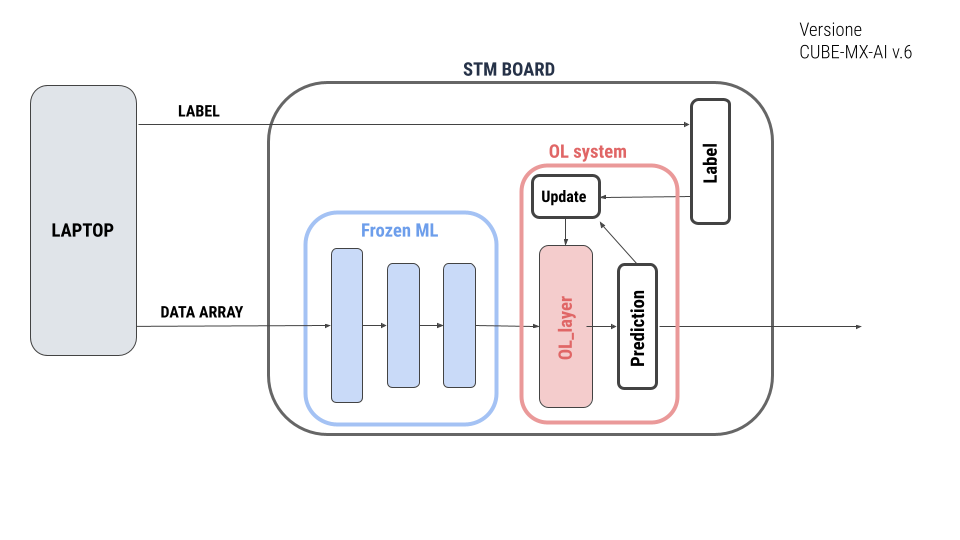
\includegraphics[width=0.7\textwidth]{Figures/Chapter3/OL.png} 
    \caption{Place holder - OL}
    \label{fig:block_diag_OL}    
\end{figure}
%
\subsubsection{TinyOL V2}

The TinyOL V2 algorithms is based on the same idea of the original TinyOL. A little intuible modification is applied in the method with the aim of contrasting catastrophic forgetting. The idea is to remove the possibility to have a drift over the original weights by removing completely this possibility. This algorithm in fact applies the same exact update rule on its parameters but it applies it only on the weights that represent the new classes. Which simply means that the rule now becomes:
    \[ w_{i,j} = w_{i,j} - \alpha (y_i - t_i) \cdot x_i \]
    \[ b_i = b_i - \alpha (y_i - t_i) \]
    \[ \text{where i=p,p+1..,n  and  j=0,1,..,m} \]
The only difference is in fact the iterator $i$, which goes from p to n, where $p$ represents the position of the first unknown class. \\
Also in thsi case the variation of the method for working on batches has been implemented. Again the algorithm is the same as TinyOL with batches but with the iterator $i$ that goes from $p$ to $n$.
    \[     W_{i,j} = W_{i,j} + \alpha (y_i - t_i) \cdot x_i\]
    \[     B_i = B_i + \alpha  (y_i - t_i) \]
And at the end of every batch the update applied on the real weights is:
    \[     w_{i,j} = w_{i,j} - \frac{1}{batch\_size} \cdot W_{i,j} \] 
    \[     b_i = b_i - \frac{1}{batch\_size} \cdot B_i \]
    \[ \text{where i=p,p+1..,n  and  j=0,1,..,m} \]
In conclusion TinyOL V2 is a simple method that differs from the original only because of a small difference in the update rule. By forcing the update on only a portion of the weight and biases the behaviour of the catastrophic forgetting that tries to modify the original knowledge and make the model drift from that context is completely removed. This helps the algorithm by contrasting catastrophic forgetting but also reduces the ability of the model to perform fine tuning on those specific classes. Another negative aspect regards the general behaviour of the final mode. By having a training strategy that updates only a portion of weights it's clear how the model itself cannot be optimized to reduce the loss function. This means that at the end of the training the model will be composed of two parts that will not work together to find the best prediction. Like before the TinyOL V2 with mini batches allows the model to learn from a bigger group of samples, this should help the model to avoid over fitting, outliers and noisy data. \\
The method TinyOL V2 requires the same amount of memory that was used by TinyOL, which means a matrix of size $n \times m$ and an array of size $n \times 1$. On the other hand the method TinyOL V2 with batches requires an additional matrix and array but this time with a reduced size of $(n-p) \times m$ and $(n-p) \times m$ since only the weight of the new classes require an update. 
%
\begin{figure}[h!]
    \centering
    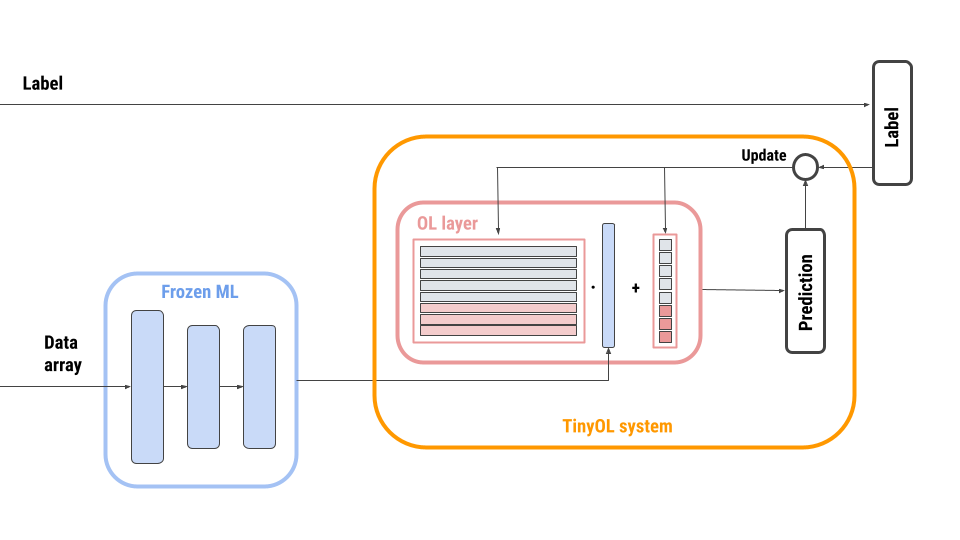
\includegraphics[width=0.7\textwidth]{Figures/Chapter3/OLV2.png} 
    \caption{Place holder - OLV2}
    \label{fig:block_diag_OLV2}    
\end{figure}
%
\subsubsection{LWF}

The LWF strategy is a regularization approach introduced in \autocite{li2017learning} and later applied with small variation in \autocite{maltoni2019continuous}. The main idea of the method is to contrast catastrophic forgetting by applying a smart loss function and double architecture that is able to combine old and new knowledge in the back propagation of the parameters. The double architecture models refers to the fact that two models are required in order to use this method. In this case the entire OL system has been applied only on the last layer of the model so the double architecture in this case is composed only of a double classification layer. The first is called $tl$, training layer while the second is called $cl$, copy layer. The role of $tl$ is to be continuously updated at each training step with the LWF back propagation rule, while $cl$ is a layer that contains a copy of all the original weights computed in the Tensorflow training, thus it represents the original knowledge of the model. The back propagation rule is based on the idea of fusing the weight updates that the two layer would apply. The fusion of these two updates is done with a weighted average that changes dynamically as the training continues. This of course implies that both layers produce a prediction, which means double computation for the OL system.\\
At this point the only major difference with respect to the TinyOL method is the double inference and the computation of the weighted back propagation. The update to be applied can be computed quite easily again by using SGD which turn out to be a simple weighted sum of two back propagation:
%
\[    \mathcal{L}_{LWF} ( y_i, z_i, t_i) =  (1-\lambda) \cdot{L}_{cross}(y_i, t_i) + \lambda \cdot{L}_{cross}(y_i, z_i) \]
\[ w_{i,j} = w_{i,j} - \alpha \cdot x_i \cdot [ (y_i - t_i)(1-\lambda) + (y_i - z_i)\lambda]  \]
\[ b_i = b_i - \alpha \cdot [ (y_i - t_i)(1-\lambda) + (y_i - z_i)\lambda] \]
\[ \text{where i=0,1..,n  and  j=0,1,..,m } \]
%
Where $y_i$ is the prediction array obtained from the layer $tl$, $z_i$is the prediction array obtained from the layer $cl$, $t_i$ is the ground truth label, $\lambda$ is the variable weight that defines which prediction has more decisional power. \\
The back propagation is composed of two parts, the first defined by $tl$ and the second defined by $cl$. The value $\lambda$ plays a very important role in this update. As explained in \autocite{maltoni2019continuous} its value cannot stay constant because it would be suboptimal. In their application the value follows a discrete function linear with the number of batches encountered, while in oiur case its value needed to be dependant on the only value known in a OL application, the amount of samples elaborated. The update of the loss function weight is the following:
\[ \lambda = \frac{100}{100+ \text{prediction$\_$counter}} \]
Another important note to be said is that in the update rule the implementation follows the variation proposed in \autocite{maltoni2019continuous}, where the loss functions ${L}_{LWF}$ used in the weighted average are not a balance between categorical cross entropy and knowledge distillation but a balance between two categorical cross entropy. This is a little modification that allows for an easier implementation without ruining the performance. \\
Also in this case a version that integrates batches is proposed. This time the method simply updates the values of $cl$ every time a batch is finished. The  algorithm this time simply becomes a fusion between old and knew knowledge where the old knowledge is refresh once in a while. In this way the model can be seen as a model that performs a weighted average in between a fast learning memory and a memory that stops in time. The size of a batch is defined by the value $k$. 
%
\[    \mathcal{L}_{LWF} ( y_i, z_i, t_i) =  (1-\lambda) \cdot{L}_{cross}(y_i, t_i) + \lambda \cdot{L}_{cross}(y_i, z_i) \]
\[ w^{TL}_{i,j} = w^{TL}_{i,j} - \alpha \cdot x_i \cdot [ (y_i - t_i)(1-\lambda) + (y_i - z_i)\lambda]  \]
\[ b^{TL}_i = b^{TL}_i - \alpha \cdot [ (y_i - t_i)(1-\lambda) + (y_i - z_i)\lambda] \]
\[ \text{where i=0,1..,n  and  j=0,1,..,m } \]
%
And at the end of a batch (once every $k$ values are elaborated):
\[ w^{CL}_{i,j} = w^{TL}_{i,j}  \]
\[ b^{CL}_i = b^{TL}_i  \]
This method, being different from the previous, requires also a different $\lambda$ rule. Experimentally it has been found to be well working an update rule defines as follows:
\begin{equation}
\lambda = \left\{
        		\begin{array}{ll}
            		1                                                         & prediction \_ counter \leq batch \_ size \\
            		\frac{\text{batch$\_$size}}{\text{prediction$\_$counter}} & prediction \_ counter >    batch \_ size
        		\end{array}
    		  \right.
\end{equation}
Both the LWF methods require the same amount of memory, which is a double prediction layer of size  $n \times m$ and $n \times 1$. Both methods are quite easy to implement and their strength is defined in the value $\lambda$ and in their update rule. They differ only from the weight updated applied on the matrix $cl$. A negative aspect that characterizes these two methods is the amount of computation required, which can be a problem for tiny devices. By having two layers and the need of two prediction is of course needed the double of computation. 
%
\begin{figure}[h!]
    \centering
    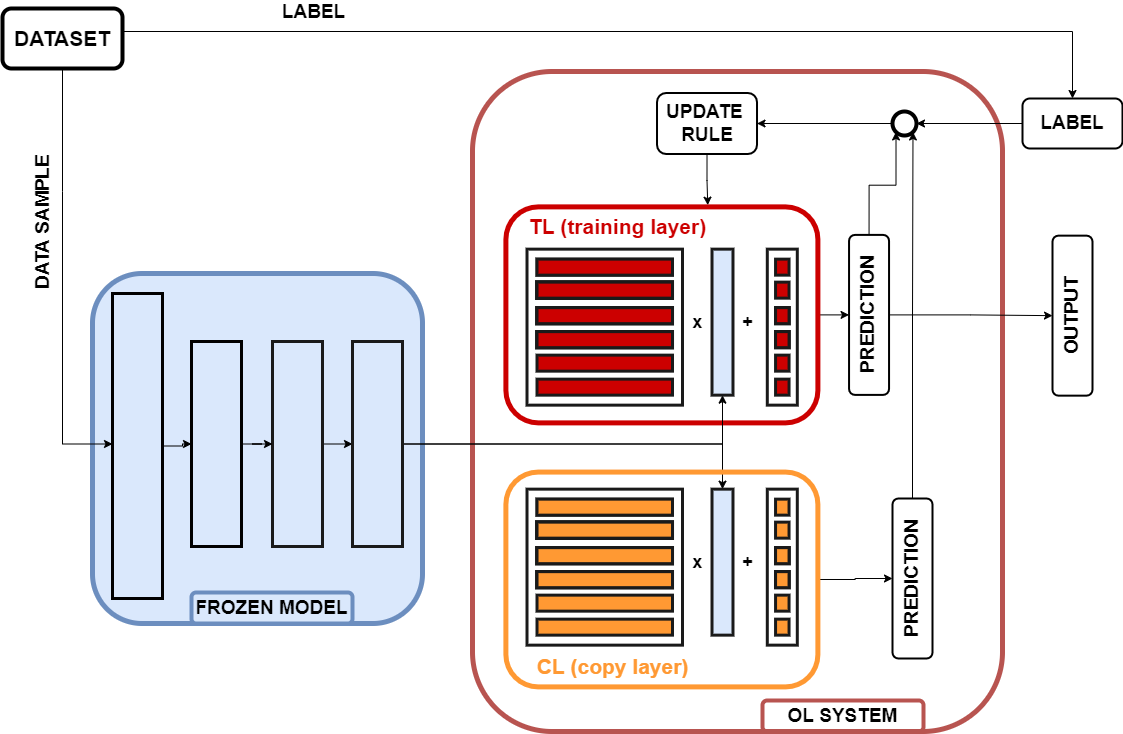
\includegraphics[width=0.7\textwidth]{Figures/Chapter3/LWF.png} 
    \caption{Place holder - LWF}
    \label{fig:block_diag_LWF}    
\end{figure}
%
\subsubsection{CWR}

CWR is an architectural approach that exploits the usage of two classification layers and a weighted back propagation rule for performing OL. Again the two classification layers are called $tl$, training layer and $cl$, consolidated layer. The idea is to perform training at each step on $tl$ with the same method as TonyOL and at the end of each batch update $cl$ with a particular rule. The back propagations for the $cl$ at the end of a batch are tge same for biases and weights and are the following:
    \[     cw_{i,j} =  \frac{cw_{i,j} \cdot updates_{i} + tl_{i,j}}{updates_{i} + 1} \] 
    \[     tw_{i,j} =  cw_{i,j}\] 
Where $tw_{i,j}$ are the weights and biases of the training layer, $cw_{i,j}$ are the weights and biases of the consolidated layer, and $updates_{i}$ is an array that behaves as a counter of labels encountered.\\
By using two classification layer that update differently the method tries to replicate the short term memory and long term memory architecture that characterizes biological brains ??? ESSERE SICURO. The layer $tl$ behaves as the short term memory since it gets updated at every single training step, and at each batch it gets reset to the correct values. The layer $cl$ behaves as a long term memory since it never gets reset or cleaned and it gets updated only once every batch with a weighted average. This weighting method depends on the number of times that a specific label appeared in the training batch.\\
Another important aspect of this method is how the prediction is computed and used. While performing only training the method requires only a prediction performed by $tl$ since this needs to get updated by its error. However if an actual prediction is requested to the model also the $cl$ layer should perform the computation and provide an inference. In fact the inference obtained by the consolidated layer is to be considered more relevant and reliable since it is produced by the long term memory. In the case a prediction is required the method needs a double prediction, one from $tl$ and the other from $cl$. Again as said for LWF this is not optimal because of the limits of tiny devices. \\
CWR is a method easy to implement. Its strength are hidden in the double architecture and the update rule that make it possible to merge short term memories and long term memories and also contrast catastrophic forgetting. The memory required for this algorithm is: to weight matrices of size $n \times m$, 2 bias arrays of size $n \times 1$, one array that keeps track of the labels encountered of size $n \times 1$. The amount of computations can change depending if a simple training step is performed or if an inference is required.
%
\begin{figure}[h!]
    \centering
    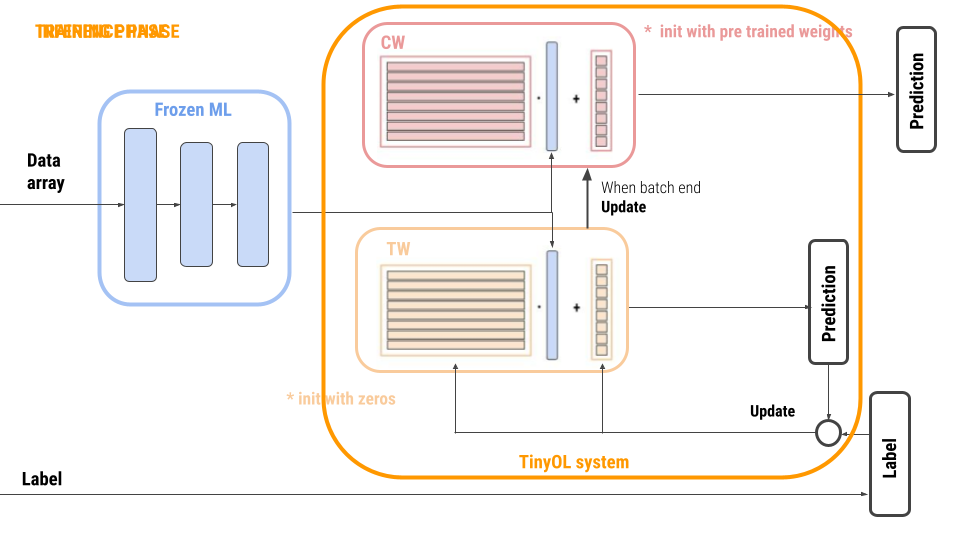
\includegraphics[width=0.7\textwidth]{Figures/Chapter3/CWR.png} 
    \caption{Place holder - CWR}
    \label{fig:block_diag_CWR}    
\end{figure}
%
\subsubsection{My algorithm}




% INSERIRE MODELLO ESEMPIO

And


\section{Gesture recognition application}

\section{Image classification application}





\chapter{Experimental setup}

In this chapter the practical aspects of the experiments are described. Initially the study has been developed entirely on the laptop using Python code with the aim of understanding the theoretical behaviour of the method and the capabilities of CL. Later the same principle and basic pipeline have been ported to the STM Nucleo and to the OpenMV camera. All applications use the same general work flow, which is: i) train the base model on a powerful device for the classification of the basic classes using Tensorflow; ii) manipulate and compress the model if necessary, then load it on the MCU of interest; iii) attach the OL system to the frozen by preparing the weights, biases, basic training parameters and the CL strategy required. \\
In this chapter all the most important steps for a good setup of the experiments are described. Starting from the dataset collection, then the training of the frozen models, then the implementation of the OL system on the MCUs and finally the application of everything on the device.

\section{Dataset collection}
In order to be able to create and train ML models it is necessary to have big datasets. In this study the two applications explored elaborate two types of data. The Nucleo F410-RE application uses time series of data recorded from and accelerometer, while the OpenMV application uses images containing the digits from the MNIST dataset. \\

\subsection{Accelerometer dataset}
For the gesture recognition study the dataset had to be created from zero. Datasets of this type, containing accelerometer data representing gestures are not very common, so it was necessary to create it. The reason that brought to this type of accelerometer data came from an example already seen during a lecture of the course Embedded Systems, where a very small dataset was used to train a ML model for the classification of vowels on an STM MCU.
The generation of the dataset has been done with the hardware described in chapter \ref{chap:hardware}, which again is a Nucelo STM32 F401-RE equipped with a shield IKS01A2 that mounts a 3D accelerometer sensor. \\
The dataset is composed of 8 different letters, which are A/E/I/O/U/B/R/M. The vowels compose the original classes that are initially learned only by the frozen model, while the three consonants are the additional classes that are learned later by the CL system. The collection of the dataset is performed by connecting the MCU to a laptop via UART protocol (USB cable). The laptop behaves as the provider of power and real time storage for the stream of data. 
For the collection of the dataset a small script that controls UART and I2C communication together with some timers and GPIOs is used. Once that a GPIO interrupt is given to the MCU and the letter is specified, the MCU starts to record the data from the accelerometer with a frequency of 100 Hz for 2 seconds. Meanwhile the data is also streamed via USB to the laptop, which stores all the data thanks to a serial communication software. In this case the software MobaXTerm was used. \\
An important note should be clarified about how the letters were drawn. To make the dataset be composed of samples that better resemble real life applications it has been decided to artificially impose an NIC scenario. This means that the samples recorded contain both new classes (the consonants) and new pattern of known classes. The latter was introduced by performing motion paths with accentuated characteristics. Some examples are the more or less oval shape of the letter O, the speed at which the sensor moves for the letter I and the general size/width/height of all letters. \\
Figure \ref{fig:letters_motion} shows the general path that was followed while drawing the letters in the air.
%
\begin{figure}[h!]
    \centering
    
\includegraphics[width=100mm]{Figures/Chapter4/letters_motion.jpg} 
    \caption{Motion of the accleerometer}
    \label{fig:letters_motion}    
\end{figure}
%
All the samples received by the MCU are saved in a table format in a text file. The columns of the table contain: the number of samples recorded, the label of the sample and three columns for the accelerations recorded from X/Y/Z axis. Since the MCU was set to work at a sampling frequency of 100 Hz for 2 seconds a single sample is composed of 600 values (200 for each axis). 
The final shape of the dataset is of 5130 samples, where the vowels have on average 560 samples each, while the consonants have circa 760 samples each. \\
Once the dataset is collected the last step of post processing is performed. This consists in a simple reshaping, shuffling and subdivision. In order to perform the training on the ML model all samples are reshaped from a matrix $3 \times 300$ to an array $1 \times 600$, which is done by stacking all the columns into a single array. After this a subdivision of the dataset is performed. Since the dataset is needed for two trainings (frozen model training and CL training), it is required to separate it correctly. The frozen model can recognize only vowels, for this reason its dataset is composed only from vowels with 176 samples from each one. The OL model is trained on all letters, so its dataset contains all the remaining vowels and all the consonants. After this, both datasets are divided in training and testing portions, which is done with the usual 80-20\% rule. Figure \ref{fig:flow_dataset_letters} shows how the dataset are divided and balanced for the two trainings.
%
\begin{figure}[h!]
    \centering
    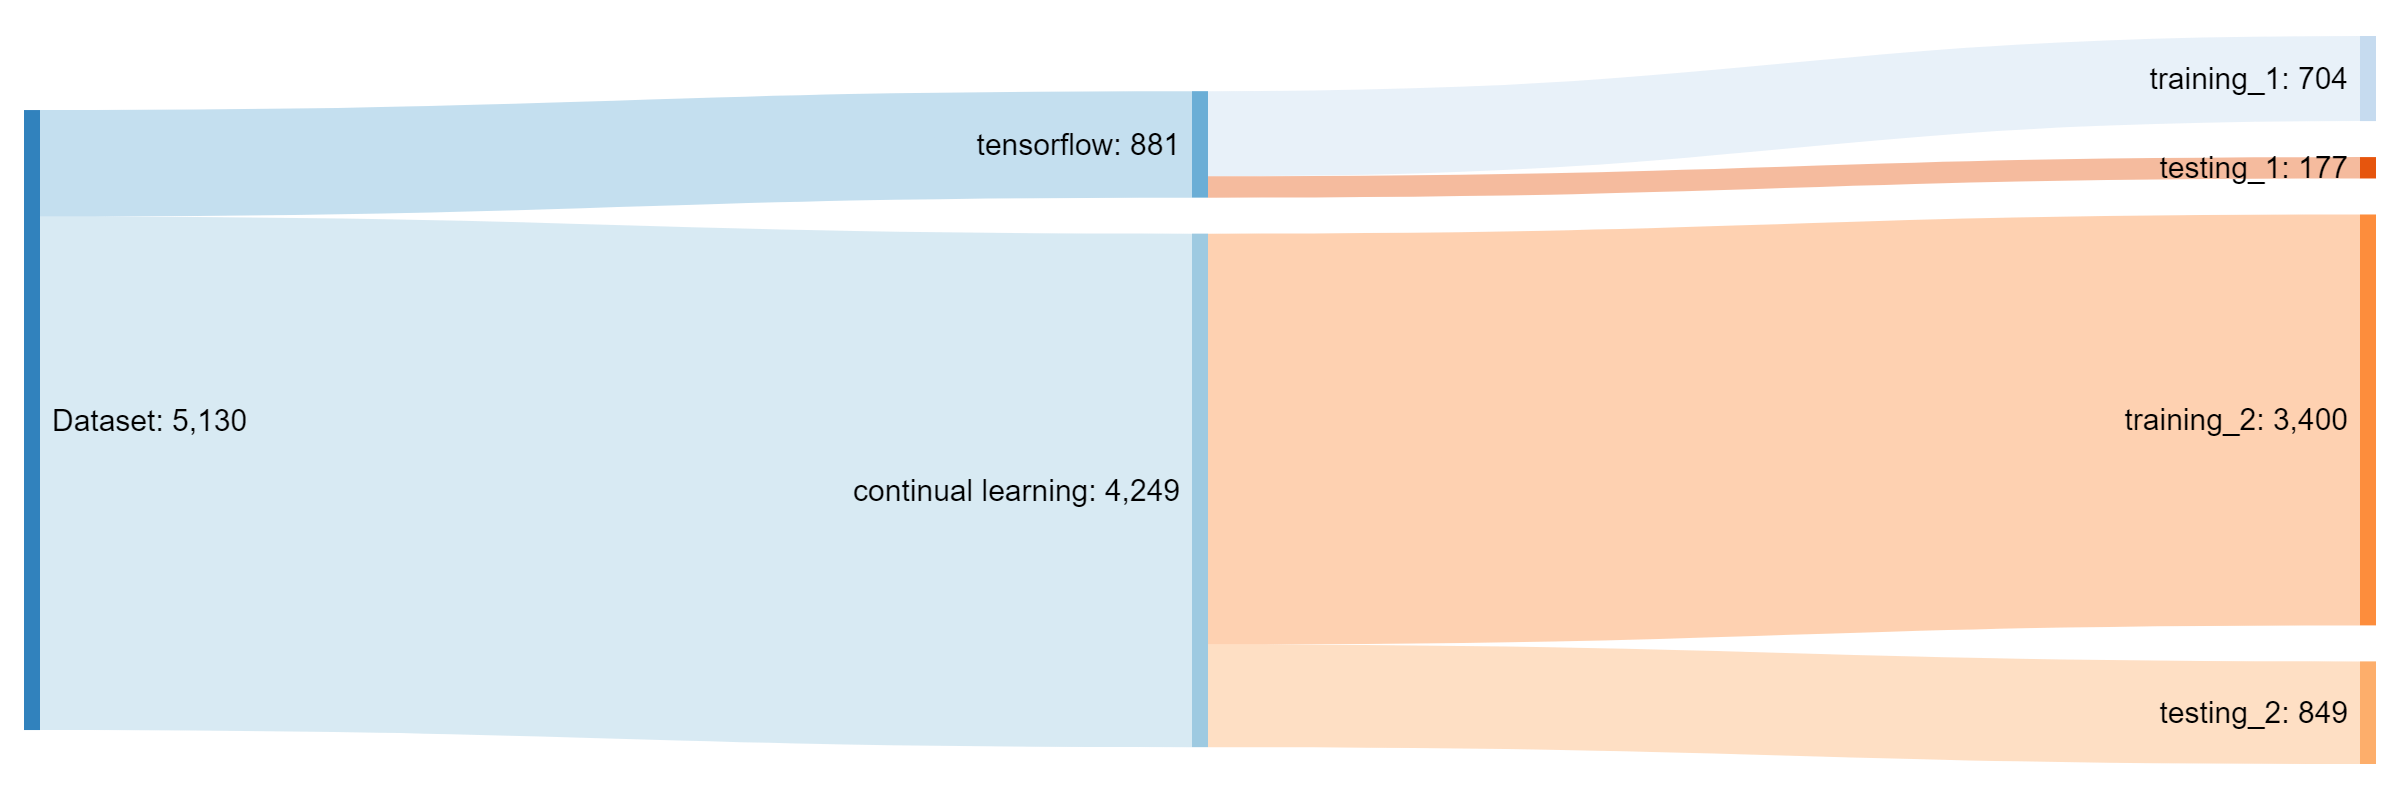
\includegraphics[width=100mm]{Figures/Chapter4/flow_dataset.png} 
    \caption{PLACEHOLDER}
    \label{fig:flow_dataset_letters}    
\end{figure}
%

\subsection{Digits recognition dataset}
For the application regarding image classification no dataset was actually required. This because it has been decided to use the well known MNIST dataset. The MNIST dataset is a publicly available large collection of photos of hand written digits. The dataset is well known in the academic and reasearch world for its small size of images and large quantity of samples. It is composed of 60000 images for training and 10000 images for testing. The images are gray scaled and have a size of $28 \times 28$ pixels. In today's research world this dataset is used a lot for training of machine learning models, especially for examples of classification or for application of generative ML models.\\
%
\begin{figure}[h!]
    \centering
    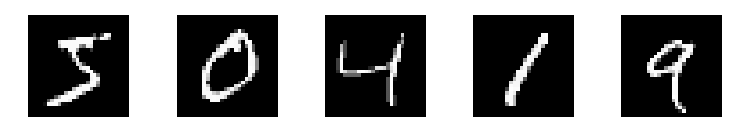
\includegraphics[width=100mm]{Figures/Chapter4/mnist_dataset.png} 
    \caption{PLACEHOLDER}
    \label{fig:mnist_dataset}    
\end{figure}
%
For the purpose of this application the dataset requires some pre processing. Since the goal of the frozen model is to correctly recognize the digits from 0 to 6 it is necessary to separate the dataset in two groups, $low\_digits$ and $high\_digits$. By doing this the $low\_digits$ group is composed of 36017 samples, while $high\_digits$ digits is composed of 23989 samples. For the training of the frozen model the entire $low\_digits$ is used in a Tensorflow training, which also requires to separate it in train, test and validate groups. For this reason the common 70-20-10 rule has been used. On the other hand for the training of the OL model only 5000 samples from the $high\_digits$ group have been used. This because from experience previously obtained from the latter application, it was demonstrated that 500 samples for each class are more than enough for a correct CL session. This dataset is then separated in training and testing with the rule 80-20\% for the CL application. \\
Figure \ref{fig:flow_dataset_openmv} shows how the dataset is divided for the training of the frozen model and OL model.
%
\begin{figure}[h!]
    \centering
    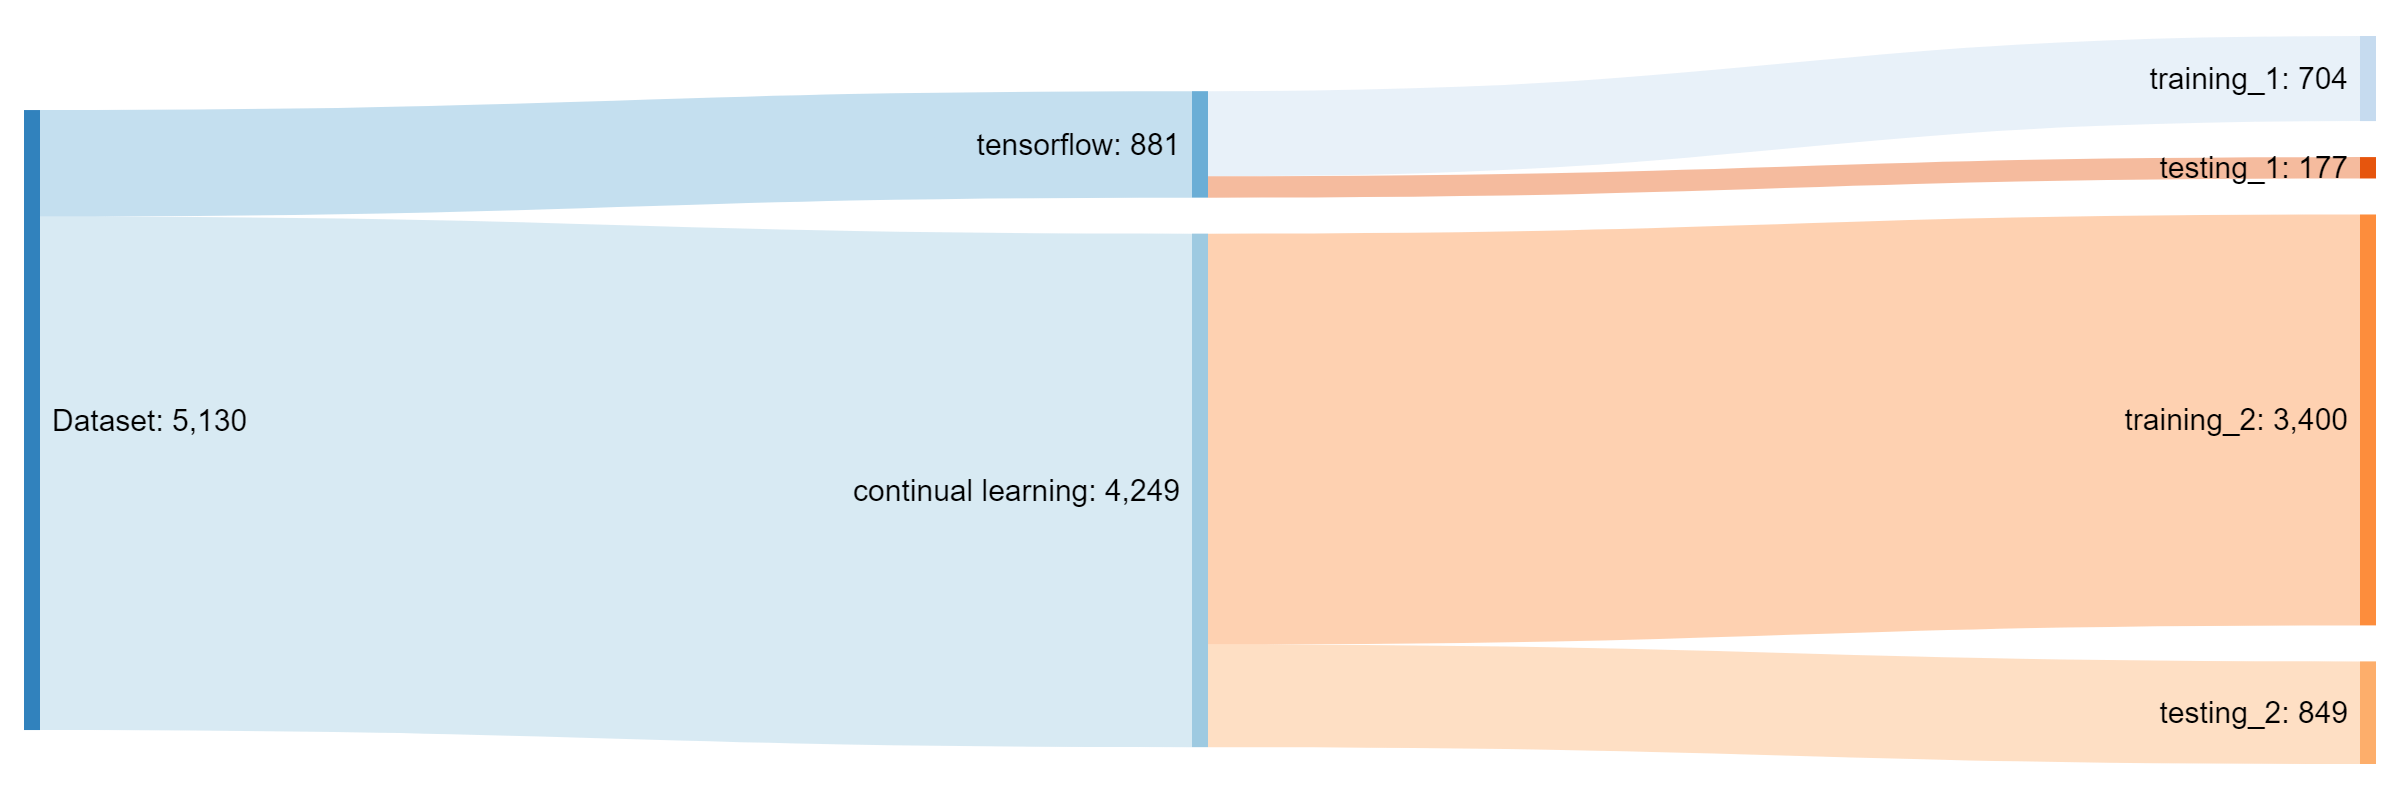
\includegraphics[width=100mm]{Figures/Chapter4/flow_dataset.png} 
    \caption{PLACEHOLDER}
    \label{fig:flow_dataset_openmv}    
\end{figure}
%


\section{Frozen model training and evaluation}
Once the dataset are created and post processed the training of the frozen models can be performed. Both models require to have an efficient structure but small in size that ensures good performances. Both performances require the use of a classification ML model, which can be achieved simply by using a Softmax activation function on the last layer. The rest of the model structure depends mainly on the elaboration required on the data. All the frozen model training was carried out with Python and Tensorflow, two very powerful and easy to use tools for machine learning. \\
The first application requires a model for the elaboration of a time series of values containing accelerometer data. Even if LSTM layers are well suited for the elaboration of data that depends on the time evolution of the signal, it has been decided to use a very simple model composed of only fully connected layer. The results brought from this simple model was satisfying enough for this application. The model is composed of 3 layers woth changing size, all characterized by ReLU as activation function execpt for the last one that uses Softmax. Figure \ref{fig:letter_structure} contains a graphic plot that shows the structure of the model.
%
\begin{figure}[h!]
    \centering
    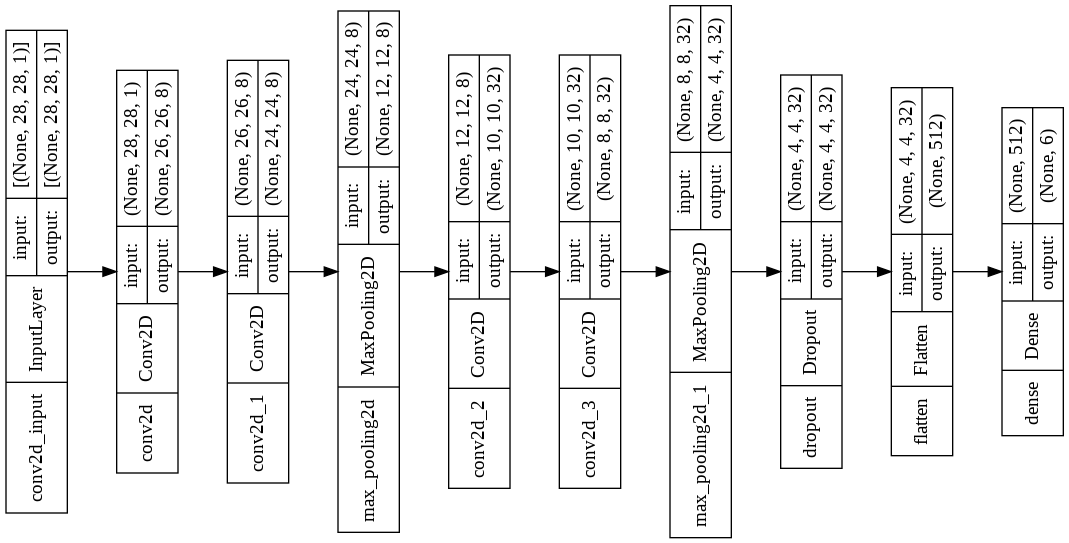
\includegraphics[width=100mm]{Figures/Chapter4/structure.png} 
    \caption{PLACEHOLDER}
    \label{fig:letter_structure}    
\end{figure}
%
The output prediction shape is of 5 classes since the classes to be predicted are just the 5 vowels.
The model's structure is quite small and simple and the number of parameters used for the training and prediction is quite limited. This type of model is well suited for an application on the Nucleo board because of its limited size. \\
The training parameters are: 
\begin{itemize}
	\item Optimizer:
	\item Loss function:
	\item Epochs:
	\item Batch size: 
	\item Test-train-validation split: 
\end{itemize}

The accuracy obtained from the testing of the model is of xxx. 
%
\begin{figure}[h!]
    \centering
    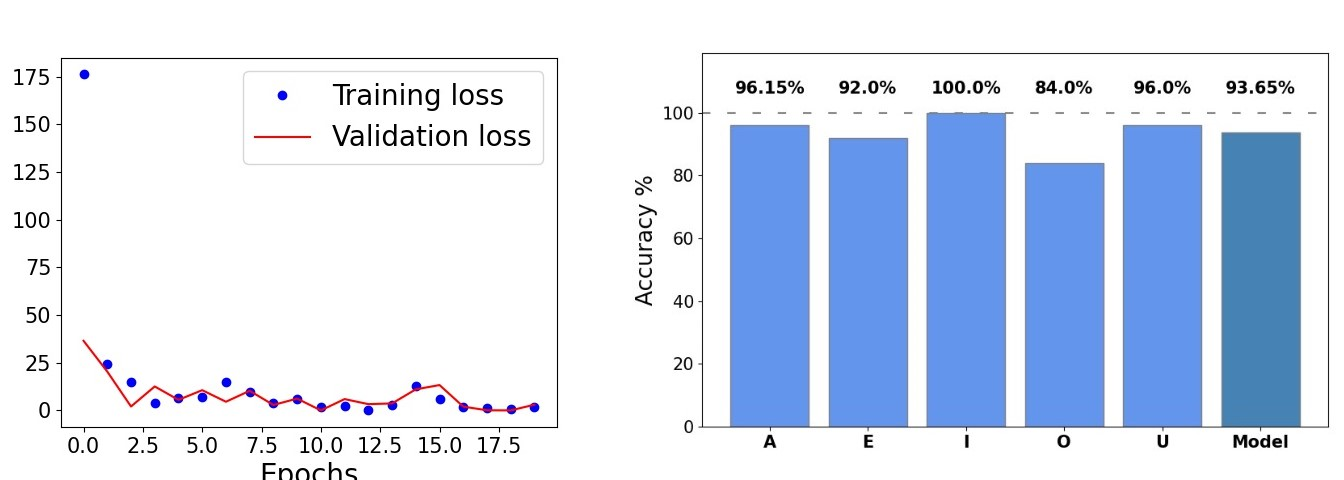
\includegraphics[width=100mm]{Figures/Chapter4/training_letters.jpg} 
    \caption{PLACEHOLDER}
    \label{fig:training_letters}    
\end{figure}
%
The second application requires the training a model for the classification of images, for this case a CNN model is better suited. The CNN structure is characterized by convolutional layer, which are purposely designed to work images. The structure of the model is the following: 
%
\begin{figure}[h!]
    \centering
    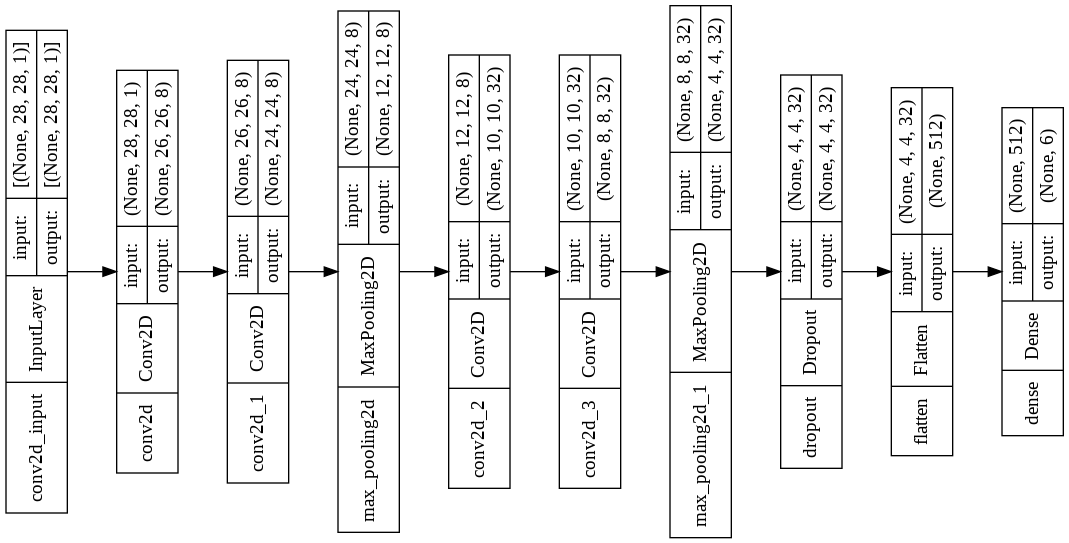
\includegraphics[width=100mm]{Figures/Chapter4/structure.png} 
    \caption{PLACEHOLDER}
    \label{fig:structure}    
\end{figure}
%
The structure contains two subsequent blocks of 2 constitutional layers followed by Max Pooling. This type of structure allows the ML model to immediatly perform feature extraction on the image. After these two block the structure is composed of a flatten layer that changes the shape of the layer from a matrix of data to an array. At this point it's possible to use a fully connected NN that actually performs the elaboration of the data and classifies it with the last Softmax layer. \\
The output prediction shape this time is of 6 classes, this beacus eth base model is required to recognize the MNIST digits 0,1,2,3,4,5. Note also how despite having a more complex structure the number of parameters in the model is not much hgher with respect to the previous application. This allows to have a small and fast model once deployed on the MCU. \\
The training parameters are:
\begin{itemize}
	\item Optimizer:
	\item Loss function:
	\item Epochs:
	\item Batch size: 
	\item Test-train-validation split: 
\end{itemize}

The accuracy obtained from the testing of the model is of $99.35\%$.
%
\begin{figure}[h!]
    \centering
    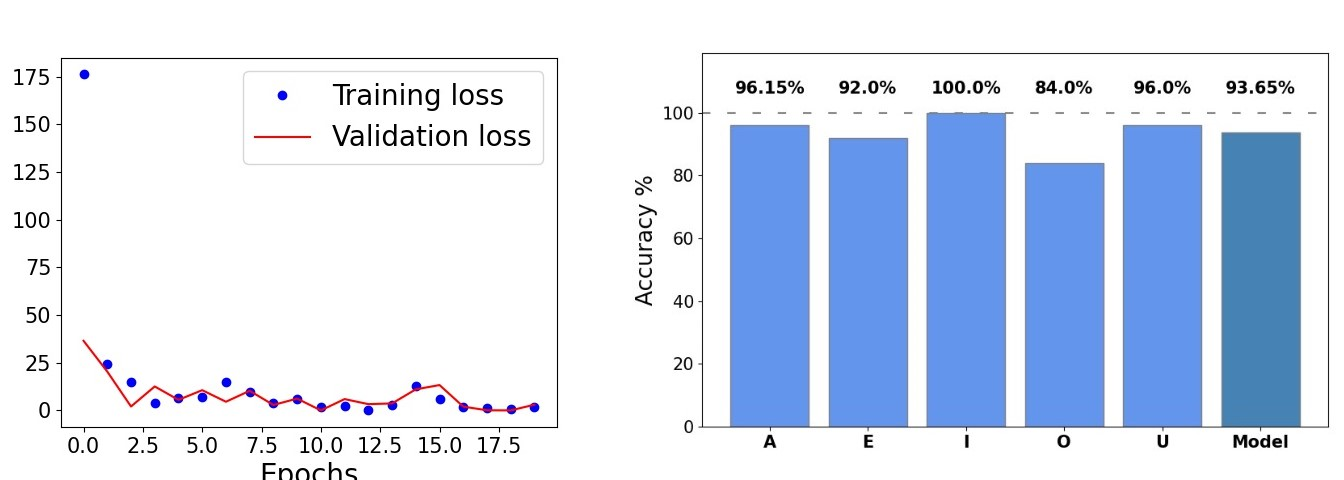
\includegraphics[width=100mm]{Figures/Chapter4/training_letters.jpg} 
    \caption{PLACEHOLDER}
    \label{fig:training_mnist}    
\end{figure}
%
Another important step that has been performed for the application on the OpenMV camera is the pruning and quantization of the model. Usually in order to deploy big models or well performing state of the art models that are not originally created for MCU use it's necessary to apply some sort of compression of the model. The most common method for doing so is a combination of pruning and quantization. Pruning is a method that tries to reduce the amount of connections in a NN model simply by putting to 0 the redundant weights thus removing the unnecessary connections. This helps in reducing the memory occupied by the model and if done strategically it can reduce the amount of computations required for the inference. In fact by injecting forced sparsity in the weights and biases it's possible to improve the efficiency and reduce the amount of computations needed. \\
For the OpenMV application a pruning operation is not actually required but it has been applied anyway in order to demonstrate the good performance of a compressed model and the potential of TinyML with complex models. Also for this operation the Tensorflow library has been used. The prunign has been set up with the following characteristics:  
\begin{itemize}
	\item Optimizer:
	\item Loss function:
	\item Epochs:
	\item Batch size: 
	\item Validation split: 
	\item Initial sparsity: 
	\item Final sparsity:
\end{itemize}

After the pruning the model is tested again and its accuracy stays very high with a value of $99.6\%$.\\
After this step it's also possible to introduce the quantization operation. This is carried out almost automatically by Tensorflow simply by calling the correct functions. The sizes of the model at the different steps of the compression are: 

% INSERRIE DIMENSIONSI FILE COMPRESSI DA PRUNING E QUANTIZATION

The last step required for the correct usage of the base model is the creation of its frozen version. As explained in section x the OL system relies on the usage of the base model as a frozen model, where its weights are not modified. In order to correctly connect to the frozen model the OL system it is necessary to remove the last layer from the frozen model and transmform it into a editable matrix od values. This can be performed easily and the final version of the frozen model is then saved as a model.h file. Then all the weights and biases of the last layer are saved in a txt file whihc will be used at deploy time from teh MCU as a start point for the CL training.  

\section{Implementation of the algorithms}
% spiegare come funziona il codice sui MCU, step principali
% spiegare l'uso degli script sul pc in real time per il training



\section{Deployment and experiment on the MCU}
% aggiungere schema a blocchi che spiega comunicazione
% aggiungere schema che mostra come è codificato il messaggio mandato da stm a pc
% aggiungere foto del training sulla openmv camera
% aggiungere foto dello schermo durante un training sulla openmv camera
In this section the process required to load all the code and models on the MCU and how to perform the experimentations are explained. At this point in the study the small framework and the models have already been created and prepared for a correct usage on the devices and just small steps are required in order to correctly use them for the applications. \bigskip
In the first experiment, the recognition of letters drawn in the air, the experiment is carried out on a Nucleo STM32 F401RE. In order to deploy the frozen model on this device, the already mentioned tool provided by STM, X-CUBE-AI, can be easily employed. The tool requires only the specification of basic parameters like the definition of the model to be loaded, the compression rateo desired and some additional info regarding validation. For this case no validation is used and no compression is applied. Once the model has been slected it is quickly checked by the tool which will display on screen informations regardin the feasibility of the usage of such model on the desired MCU board. Once this is done the model is loaded in the board and inference can now be performed quite easily by leveraging all the efficient functions provided by the extension pack of STM. \\
At this point the experiment can be carried out. Instead of having a very long and tedious training performed by a user that keeps recording acclelerometers motion with the MCU in his had it has been decided to feed to the device the data from the computer. In order to do so a small app runnin on Python has been developed. The app exploits the usage of pyserial, a library used for serial communication (UART protocol) via USB cable and it's able to stay in sync with the device and continuosly send and recieve information. 
The script is divided in x small sections: initially it loads all the arrays of accelerometer data that has been previously saved in a txt file, then it prepares the serial port for the communication by setting the correct parameters, then it initializes some data containers used for saving the performance of the model in real time, then an infinite while loop starts where the actual communication between the devices is performed, here a sort of state machine is used for performing training or testing. 
The communication is quite easy, when the python script is launched an infinite loop starts, here the script wait for an acknowledgement from the device that will let it know that the training is starting. Once the signal is received the sends the data packets used for the training. The data packets are just a string of 600 values that represent the accelerometer values from the three axis and a char value that represents the ground truth label. The training step is then performed on the MCU and once finished the MCU responds tot he laptop with a small message of ust 32 bytes containinginfornations regarding the inference and training step performed. Once the responce is sent and received the STM will again send an ackoledgment signla that lets the laptop know that a new traingn step is starting, thus a new data sample is requested. At this point the entire communication procedure repeats. 
The trainings continues until the device reaches the testing section. Here the communication the only thing that changes is the fact that the laptop is going to save in the previously generated containrs the informations related to the training. This allows the laptop to later draw some conclusions about the training performance and the model accuracy at thsi time of the application. \\
A complete training procedure lasts for about 10 minutes, and at the end of the procedure the python script will automatically generate some bar plots containing the accuracy of each class, a confusion matrix and a table containing relevant informations. \bigskip
The application on the OpenMV camera is quite similar. Once the model and the required additional information are prepared eveyrthing can be loade don the MCU. This time in order to load the ML model on the camera a toolchain provided by STM is used. This toolchain is installed in a virtual machine runnin gon Ubuntu OS that has been provided by the University lab. Thanks to these tools it's possible to generate a new firmware that will contain the structure of the ML model and it's then immediate to load this file on the camera itself.  \\
At this point the code correct main.py file should be loaded on the camera together with the library created and two files containing the weights from the last layer. Again as before, in order to provide a fast, easy to repeat and reliable training a small computer app running on Python has been developed. The app requires the usage of three main libraries, PySerial, Tensorflow and OpenCV. The first one is used for loading correctly the dataset of MNIST digits images because these are avilable only from there. The PySerial library is necessary for the control over the transmission of data that happens over USB cable. The OpenCV library is insted used only for display purposes. The generic ode of the app cna be divided in blocks: initially load the entire MNIST dataset and extract a balanced subset of the dataset that contains the requested amounf of images from each digit, open two windows on the screen that are used for seeing in real time what the camera is catching in real time and for displaying the digits from the MNIST, then simply use the UART protocol to connect to the camera, enter in the infinite while loop and perform the transission depengin on the state requested by the laptop. \\
The communication is again based on the UART protocol. At first the COM port is set by the script in order to use perform correctly the transmission. After that the script sends a small message of 4 chars to the MCU. Dependnin gon the word written inside this message the camera behaves in different ways. If the word is $snap$ then the camera simply takes a photo, compresses it and sends it back to the laptop that will then use OpenCV to display it inside one of the opened windows, if the messgae is $elab$ then the camera performs the same action as $snap$, but the laptop this time will slowly change the displayed MNIST digits from 0 to 9. This is done to be sure that the camera is correctly oriented on the windows and be sure that the entire digits is captured in the photos. FInally if the message contains the word $trai$ then the camera is set to perform the OL training. In this state the camera will immediately wait for another messge containin gonyl a char, which represents the ground truth label and then will start the training step of the OL procedure. In order to maintain sync with the laptop the camera will not also send the captured and compressed image over serial communication. SO once the training step is finished the camera waits until the next label is received. This time the app doesn't work on ACK signals but works on small waiting times. Once the entire training and testing is done the camera saves all the informatins related to the performance inside a txt file that is then stored in the SD card. In order to create some plots and tables it's necessary to run an external script on the copy pasted informations. 



\section{Gesture recognition setup}

\section{Image classification setup}






\chapter{Experimental results} 

\section{Experiment A: Gesture recognition}

\section{Experiment B: Image classification}

This section contains and explains the results obtained from the test performed. Initially a description about the comparison between simulation and real application is performed with the aim of understanding if the training on the nucleo evolves as the simulation on the laptop. Then the results obtained from the application from the Nucleo are discussed and finally the results from the OpenMV application are described.\\
To understand if the Nucleo STM32 F401-RE is able to perform a real time ML training a study concerning the history of its parameters is done. The idea is to record the variation of the most important parameters from the OL layer at every training step and then compare its evolution to the same parameter evolutioin but recorded from the simulation carried out on the laptop. The parameters of interest are the biases of the OL layer, the predictions obtained from Softmax, the output of the frozen model, 10 weights picked randomically from the weight matrix. The evolution of the parameters is then displayed in a plot with the aim of observing how and if the history recorded from the laptop differs from the history recorded from the MCU. This is done qualitatively simply by looking at superimposition of the two lines. Figure \ref{fig:comparison_frozen} shows one example of comparison for the frozen model outpus, figure \ref{fig:comparison_bias} shows the comparison of the bias evolution, figure \ref{fig:comparison_weights} shows the comparison of the weights evolution, figure \ref{fig:comparison_softmax} shows the difference of the predictions obtained from Softmax.
%
\begin{figure}[h!]
    \centering
    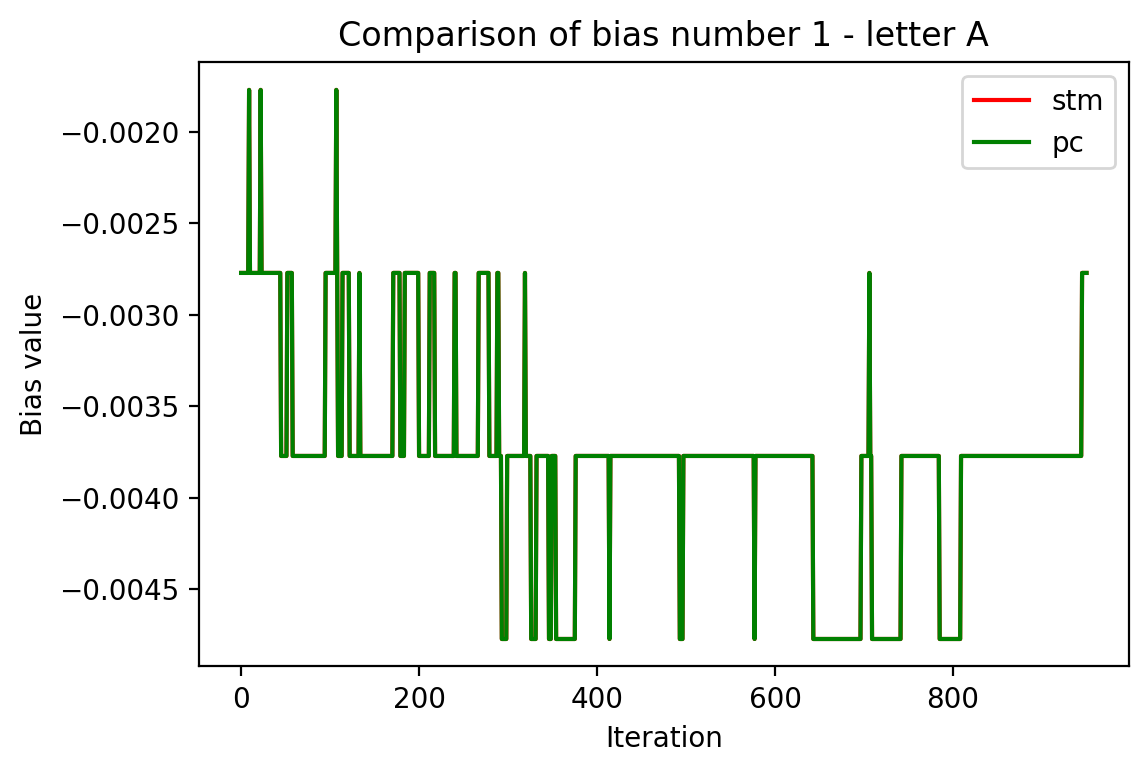
\includegraphics[width=100mm]{Figures/Chapter5/bias_example.png} 
    \caption{PLACEHOLDER}
    \label{fig:comparison_bias}    
\end{figure}
%
%
\begin{figure}[h!]
    \centering
    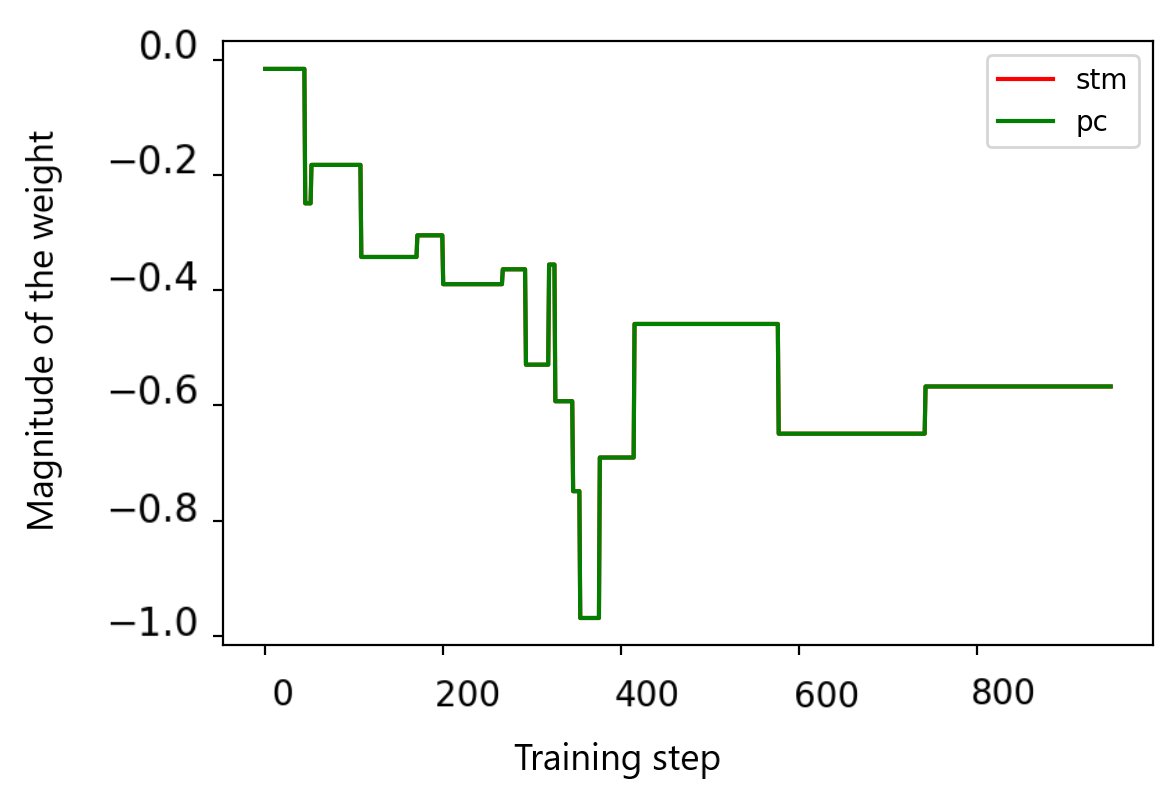
\includegraphics[width=100mm]{Figures/Chapter5/weight_example.png} 
    \caption{PLACEHOLDER}
    \label{fig:comparison_weights}    
\end{figure}
%
%
\begin{figure}[h!]
    \centering
    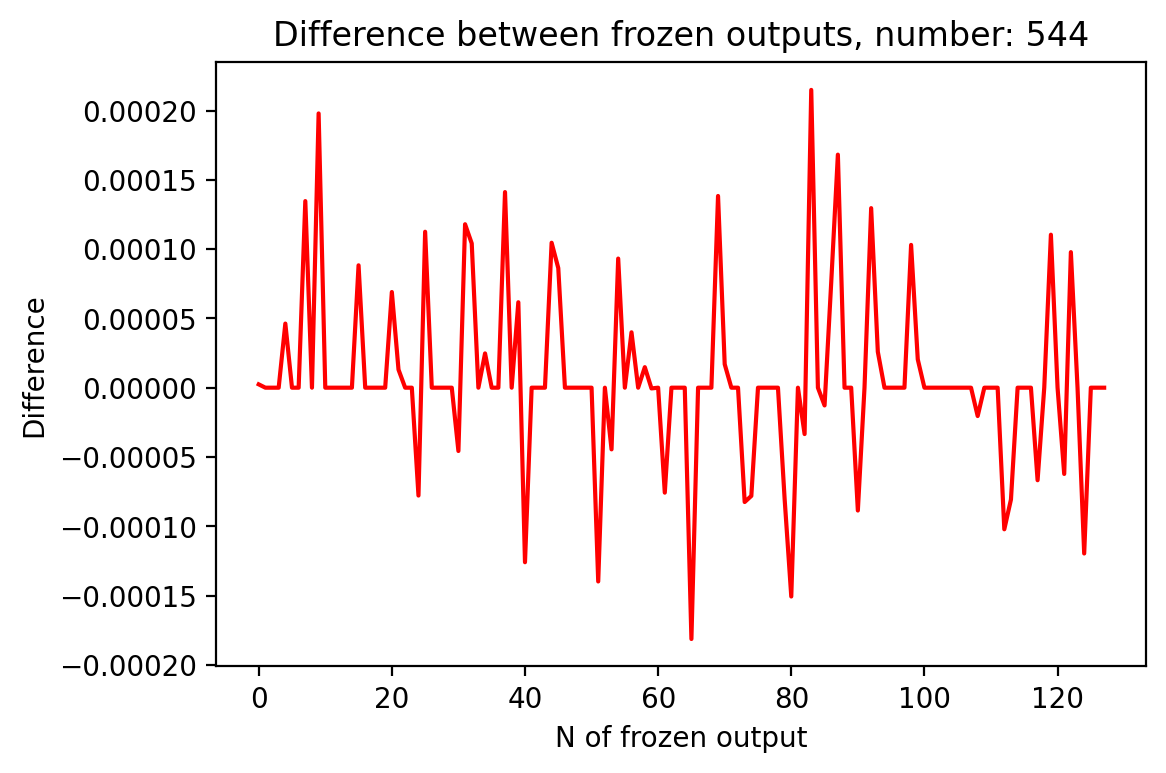
\includegraphics[width=100mm]{Figures/Chapter5/frozen_example.png} 
    \caption{PLACEHOLDER}
    \label{fig:comparison_frozen}    
\end{figure}
%
%
\begin{figure}[h!]
    \centering
    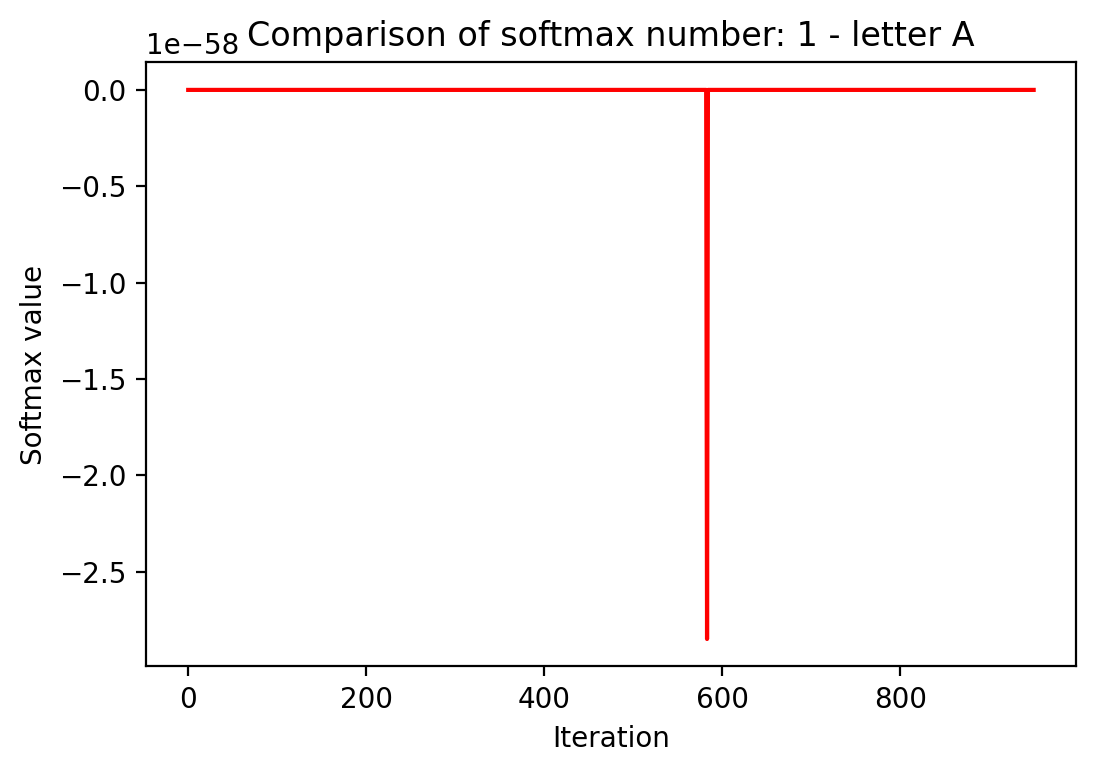
\includegraphics[width=100mm]{Figures/Chapter5/softmax_example.png} 
    \caption{PLACEHOLDER}
    \label{fig:comparison_softmax}    
\end{figure}
%
The plots displayed above are examples of the evolution performed, but they are rappresentative of the behaviour of all parameters. It's clear from the results how the two applications are very close, differencing from each other by just a small magnitude and for very few training step. Only one difference can be noted in figure x, where the dofference of the softmax prediction is dofferent from zero but still very little. This error in fact doesn't introduce any problem in the evolution since in the following steps the error goes back to 0. \\
One of the main concerns was about the feature extraction performed by the frozen model. Because of the limited resources of the MCU usually models are compressed to be later loaded on the device. In this case no pruning or quantization have been applied, so the frozen model loaded on the MCU and laptop are exactly the same. The concern regards how the prediction is carried out by the X-CUBE-AI tool on the MCU compared with Tensorflow on the laptop. Figure \ref{fig:comparison_max} contains two examples of comparison of frozen model outputs. The x axis contains the iterator representing the i-th difference computed between the i-th value from the Tensorflow and STM output from the frozen model. On the left the difference that contains the biggest error is displayed, while on the right is displayed the sample that contains the second biggest error. It's clear how the plot on the left is not a correct representation of the MCU behaviour since it has a magnitude far too high when compared to the second biggest error.
%
\begin{figure}[h!]
    \centering
    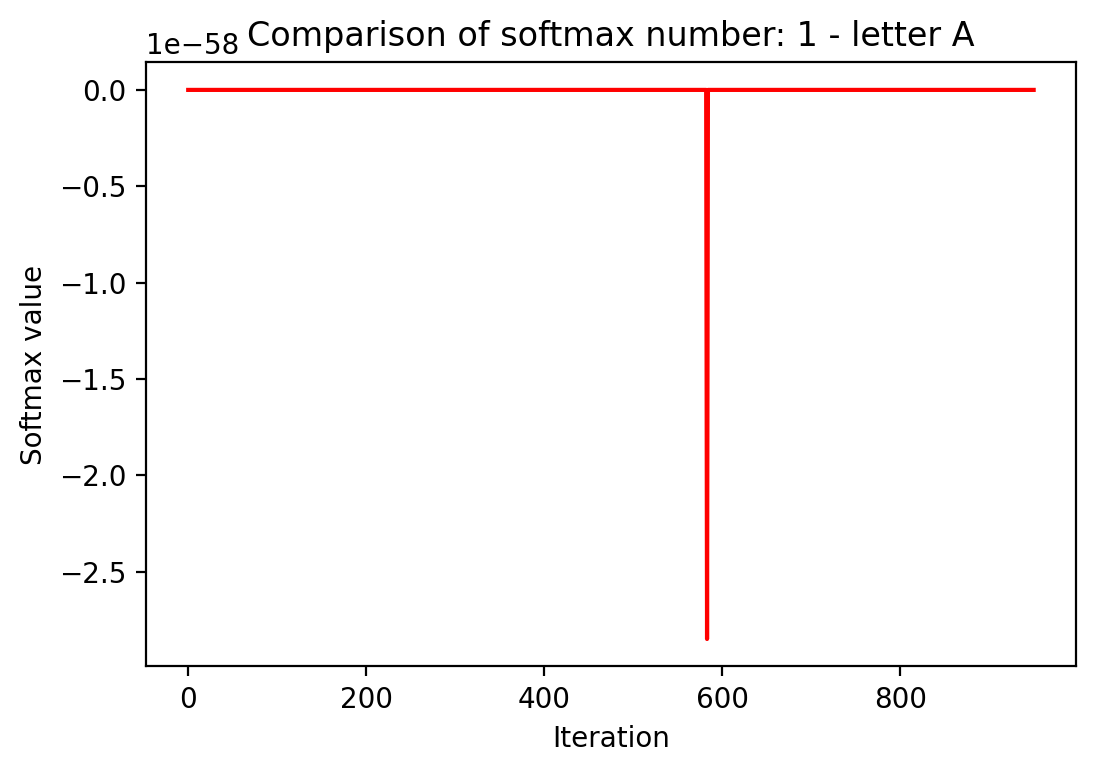
\includegraphics[width=100mm]{Figures/Chapter5/comparison_difference.png} 
    \caption{PLACEHOLDER}
    \label{fig:comparison_max}    
\end{figure}
%
Thanks to this study it is possible to conclude that a training performed on such a small device is actually possible and in terms of accuracy and precision it is as reliable as a training performed on a powerful device. Because of these plots it is then possible to conclude that the evolution of the model on the MCU is reliable and correct. A model trained on such device is subject to the same exact evolution that would affect the model in the case the training were to be carried on a laptop. From this point on all the experiment and results are obtained from MCUs.
\bigskip

Speaking about the gesture recognition experiment once the training have been carried out it's possible to display the accuracy of every single algorithm for every single class. As mentioned in section REFERENCE SECTION the testing is performed on the last 20 \% of the dataset, so on a total of XXX samples. The bar plots containing the accuracies from every strategy together with their confusion matrices are displayed in Figures \ref{fig:letter_res_OL} \ref{fig:letter_res_OL_batch} \ref{fig:letter_res_OL_v2} \ref{fig:letter_res_OL_v2_batch} \ref{fig:letter_res_LWF} \ref{fig:letter_res_LWF_batch} \ref{fig:letter_res_CWR}.  
%
\begin{figure}[h!]
    \centering
    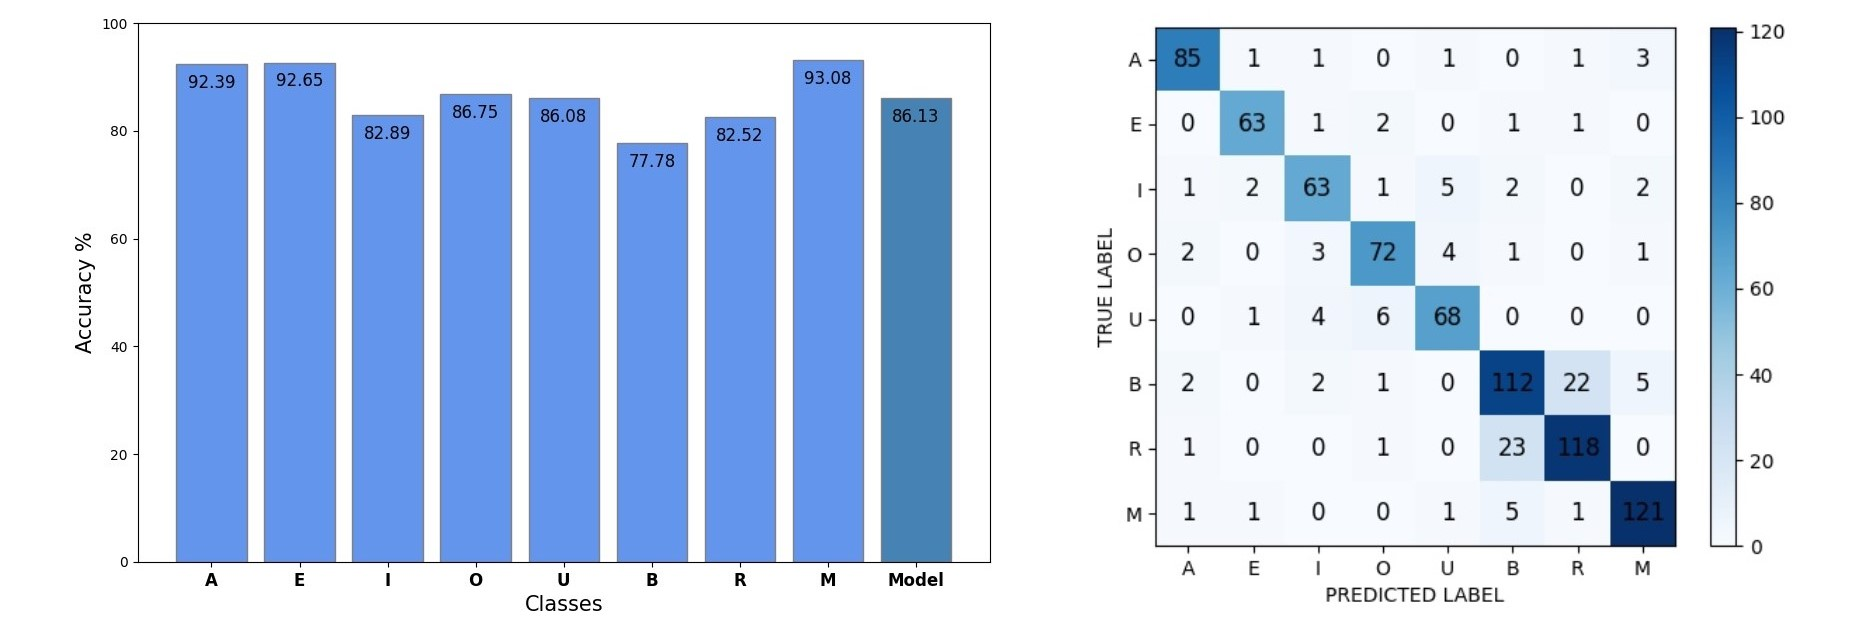
\includegraphics[width=100mm]{Figures/Chapter5/STM_barPlot_OL.jpg} 
    \caption{PLACEHOLDER}
    \label{fig:letter_res_OL}    
\end{figure}
%
%
\begin{figure}[h!]
    \centering
    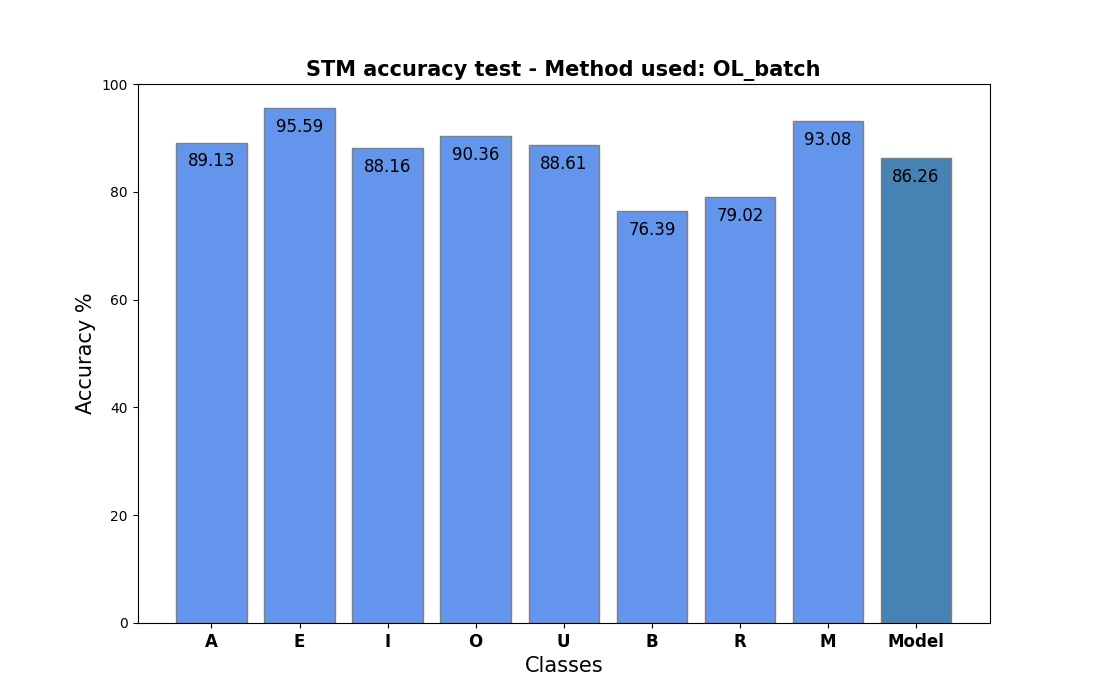
\includegraphics[width=100mm]{Figures/Chapter5/STM_barPlot_OL_batch.jpg} 
    \caption{PLACEHOLDER}
    \label{fig:letter_res_OL_batch}    
\end{figure}
%
%
\begin{figure}[h!]
    \centering
    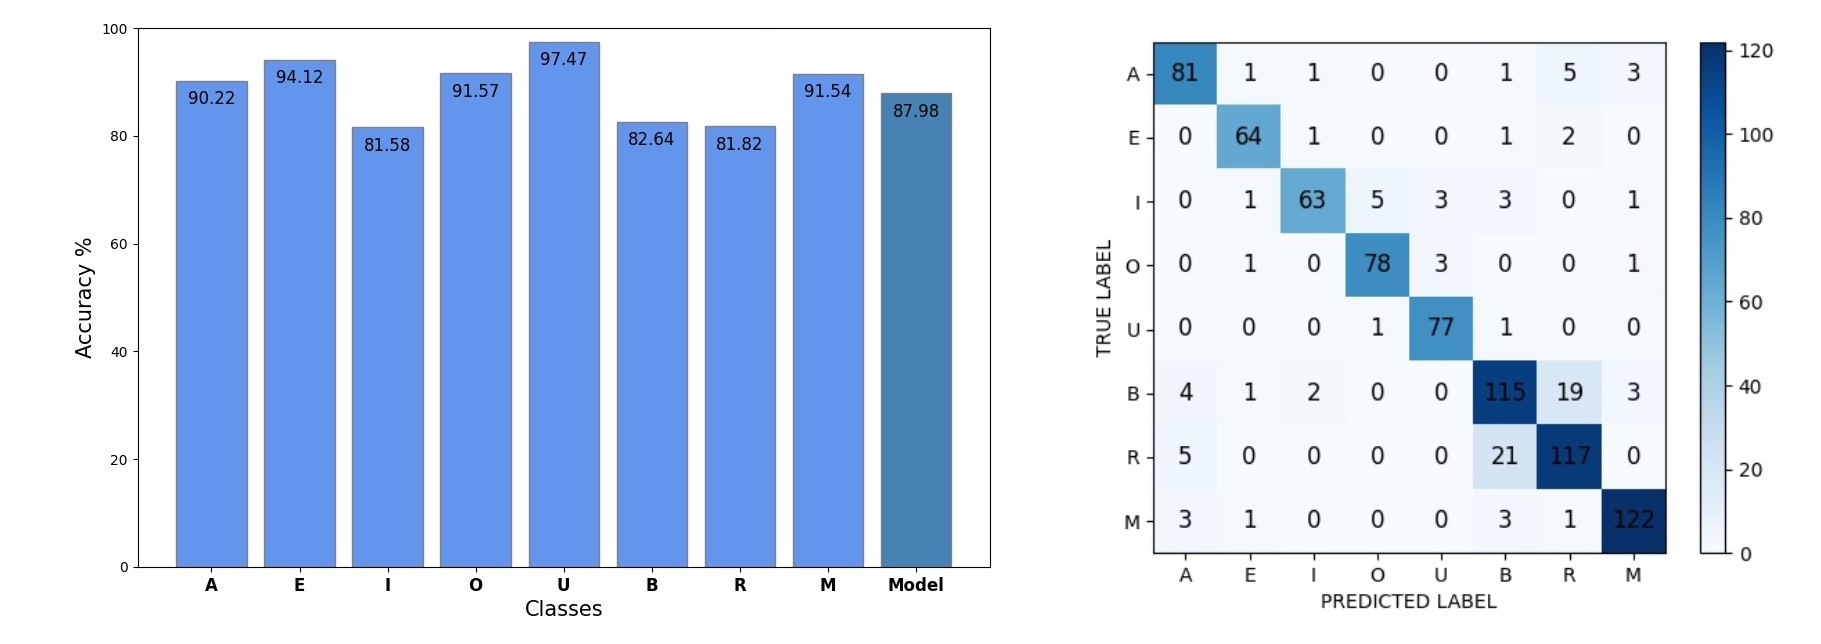
\includegraphics[width=100mm]{Figures/Chapter5/STM_barPlot_OL_V2.jpg} 
    \caption{PLACEHOLDER}
    \label{fig:letter_res_OL_v2}    
\end{figure}
%
%
\begin{figure}[h!]
    \centering
    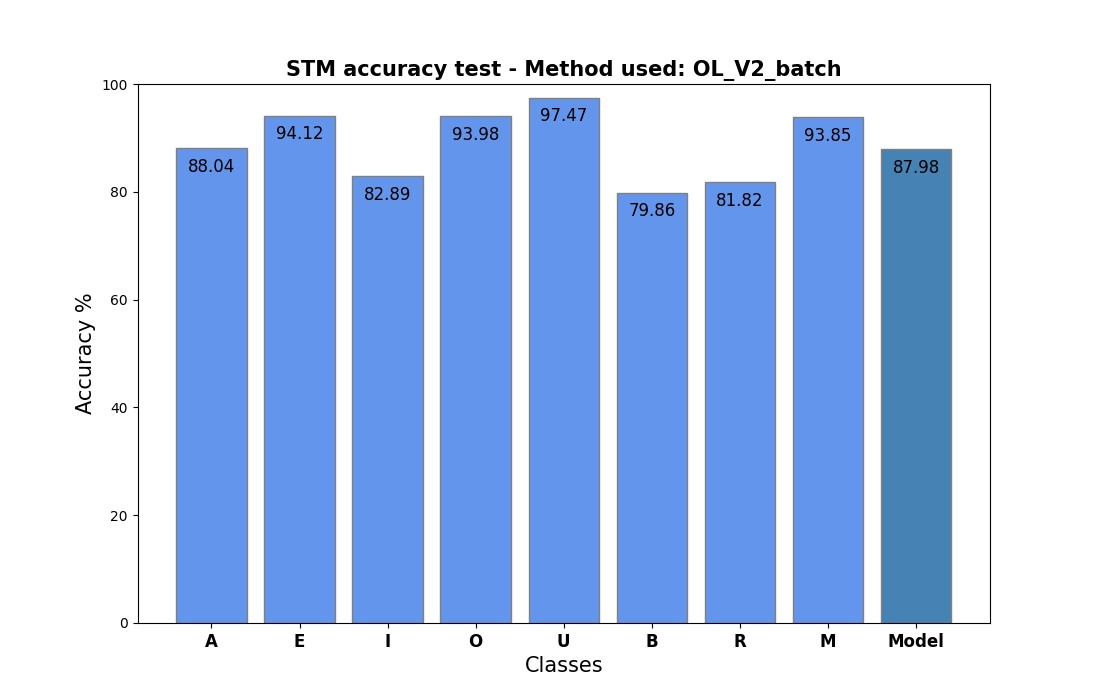
\includegraphics[width=100mm]{Figures/Chapter5/STM_barPlot_OL_V2_batch.jpg} 
    \caption{PLACEHOLDER}
    \label{fig:letter_res_OL_v2_batch}    
\end{figure}
%
%
\begin{figure}[h!]
    \centering
    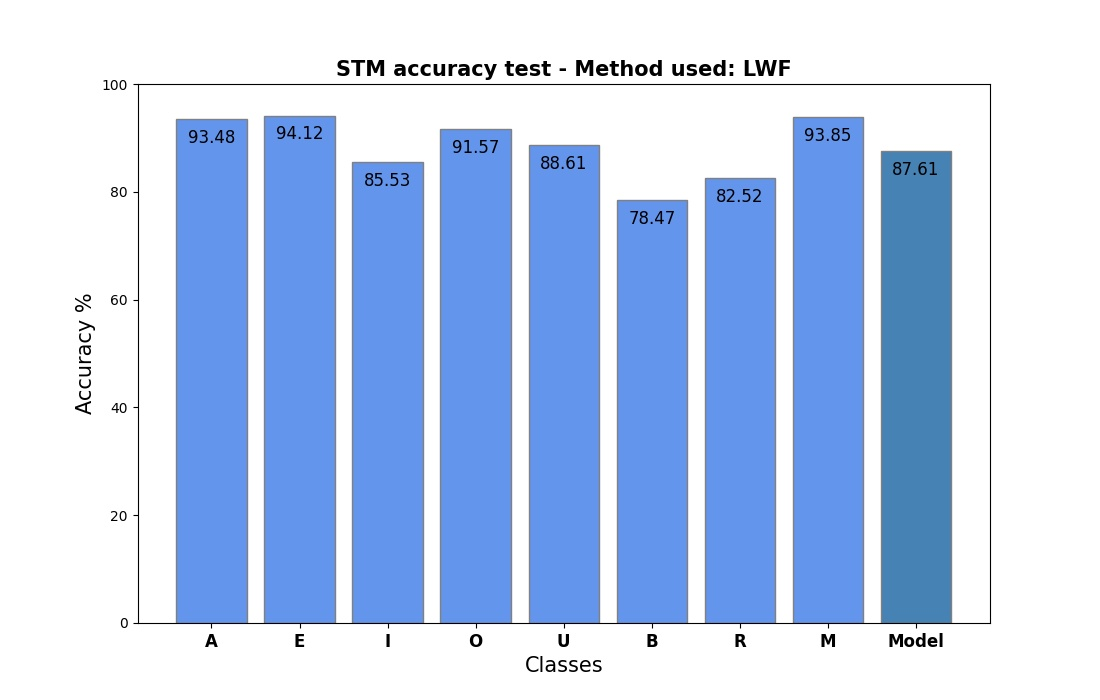
\includegraphics[width=100mm]{Figures/Chapter5/STM_barPlot_LWF.jpg} 
    \caption{PLACEHOLDER}
    \label{fig:letter_res_LWF}    
\end{figure}
%
%
\begin{figure}[h!]
    \centering
    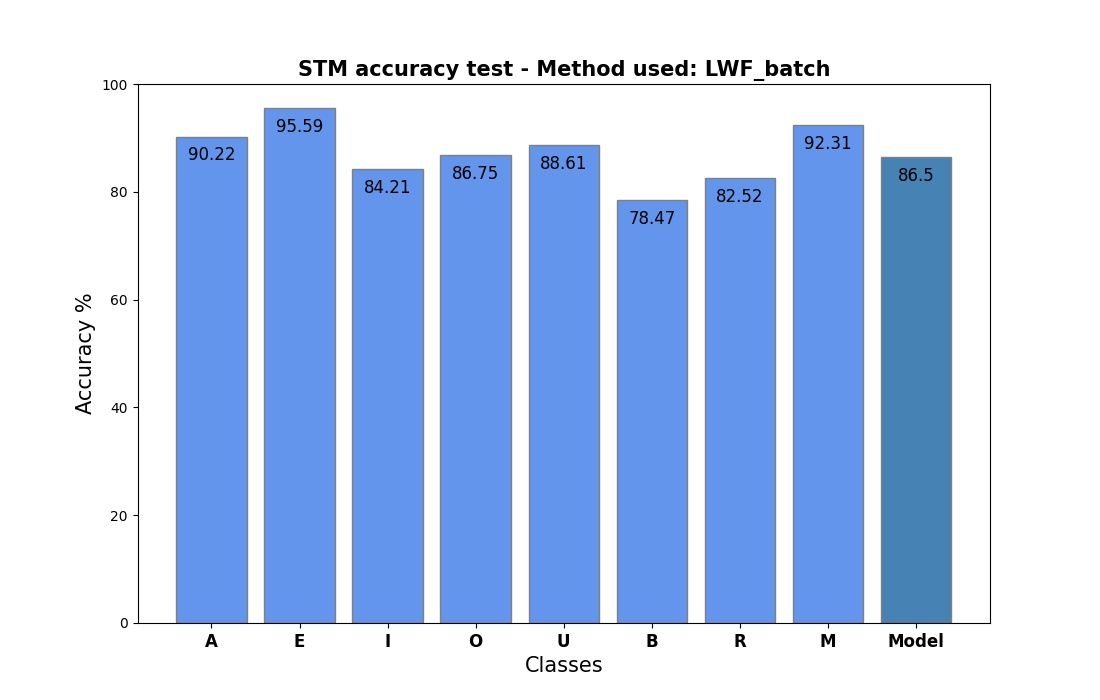
\includegraphics[width=100mm]{Figures/Chapter5/STM_barPlot_LWF_batch.jpg} 
    \caption{PLACEHOLDER}
    \label{fig:letter_res_LWF_batch}    
\end{figure}
%
%
\begin{figure}[h!]
    \centering
    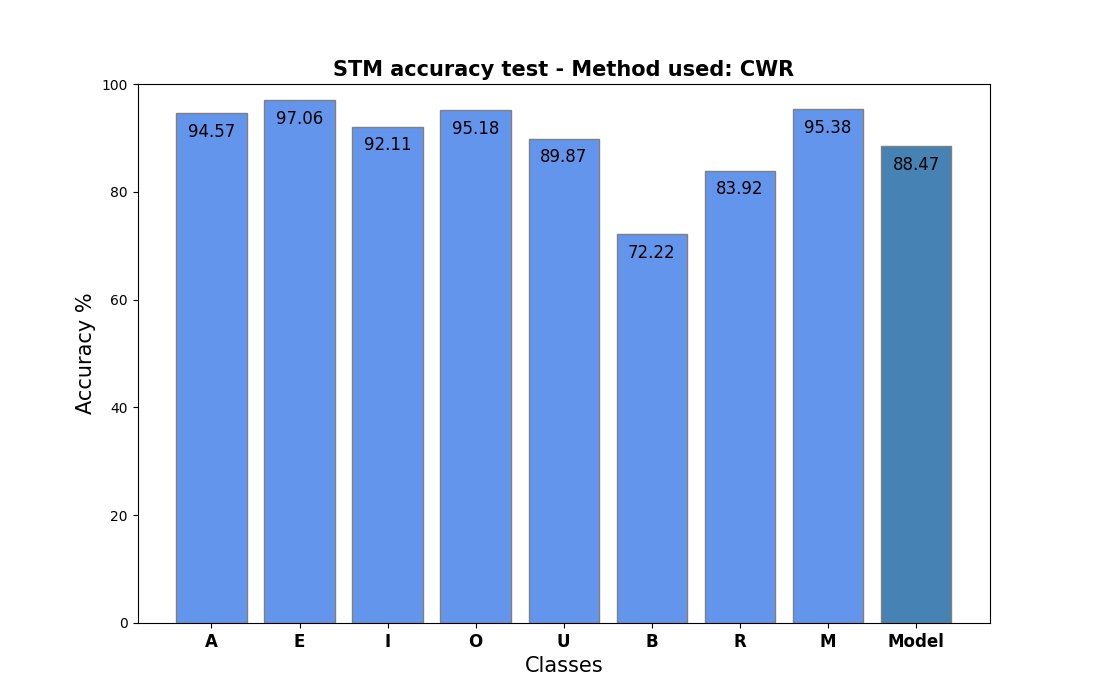
\includegraphics[width=100mm]{Figures/Chapter5/STM_barPlot_CWR.jpg} 
    \caption{PLACEHOLDER}
    \label{fig:letter_res_CWR}    
\end{figure}
%
From these plots it is clear how all methods are quite good in digesting new classes and completely fuse them in the classification layer. No method in fact shows a bad learning on a specific class exept for the letter B that in all methods sees a lower accuracy when compared to others. It' easy to see from the cofusion matrix that the letter is not learned in a wrong way but rather the letter is easily confused with the letter R. Most probably this is because the path that has been followed when the dataset has beenc reated differs for just the leg of letter R. \\
Table x and table x contain other important results from the experiment. 
%
\begin{table}[]
\begin{center}
\begin{tabular}{l|cccc}
                     & \multicolumn{1}{c|}{\textbf{Accuracy \%}} & \multicolumn{1}{c|}{\textbf{\begin{tabular}[c]{@{}c@{}}Average time\\ inference frozen\\  model in ms\end{tabular}}} & \multicolumn{1}{c|}{\textbf{\begin{tabular}[c]{@{}c@{}}Average time \\ inference OL\\ layer in ms\end{tabular}}} & \multicolumn{1}{c|}{\textbf{\begin{tabular}[c]{@{}c@{}}Maximum allocated \\ RAM in kB\end{tabular}}} \\ \hline
\textbf{OL}          & 86.13                                     & 10.65                                                                                                                & 0.99                                                                                                             & 26.1                                                                                                 \\ \cline{1-1}
\textbf{OL batch}    & 86.26                                     & 10.65                                                                                                                & 1.54                                                                                                             & 29.8                                                                                                 \\ \cline{1-1}
\textbf{OL V2}       & 87.98                                     & 10.65                                                                                                                & 1.03                                                                                                             & 26.1                                                                                                 \\ \cline{1-1}
\textbf{OL V2 batch} & 87.98                                     & 10.65                                                                                                                & 1.11                                                                                                             & 29.8                                                                                                 \\ \cline{1-1}
\textbf{LWF}         & 87.61                                     & 10.65                                                                                                                & 3.45                                                                                                             & 29.9                                                                                                 \\ \cline{1-1}
\textbf{LWF batch}   & 86.5                                      & 10.65                                                                                                                & 3.26                                                                                                             & 29.9                                                                                                 \\ \cline{1-1}
\textbf{CWR}         & 88.47                                     & 10.65                                                                                                                & 2.11                                                                                                             & 29.9                                                                                                 \\ \cline{1-1}
\textbf{MY ALG}      & 86.87                                     & 10.65                                                                                                                & 3.54                                                                                                             & 29.9                                                                                                 \\ \cline{1-1}
\end{tabular}
\end{center}
\end{table}
%
\begin{table}[]
\begin{tabular}{cc|cccccccccc}
\multicolumn{1}{c|}{\multirow{2}{*}{Algorithm}} & \multirow{2}{*}{Parameter} & \multicolumn{8}{c|}{Class}                                                                                                                                                                            & \multicolumn{1}{c|}{\multirow{2}{*}{\begin{tabular}[c]{@{}c@{}}batch\\ size\end{tabular}}} & \multirow{2}{*}{\begin{tabular}[c]{@{}c@{}}learning\\ rate\end{tabular}} \\
\multicolumn{1}{c|}{}                           &                            & \multicolumn{1}{c|}{A} & \multicolumn{1}{c|}{E} & \multicolumn{1}{c|}{I} & \multicolumn{1}{c|}{O} & \multicolumn{1}{c|}{U} & \multicolumn{1}{c|}{B} & \multicolumn{1}{c|}{R} & \multicolumn{1}{c|}{M} & \multicolumn{1}{c|}{}                                                                      &                                                                          \\ \hline
\multirow{3}{*}{OL}                             & Accuracy                   & 0.92                   & 0.93                   & 0.83                   & 0.87                   & 0.86                   & 0.78                   & 0.83                   & 0.93                   & \multirow{3}{*}{16}                                                                        & \multirow{3}{*}{16}                                                      \\ \cline{2-2}
                                                & Precision                  & 0.92                   & 0.93                   & 0.85                   & 0.87                   & 0.86                   & 0.78                   & 0.83                   & 0.92                   &                                                                                            &                                                                          \\ \cline{2-2}
                                                & F1 score                   & 0.92                   & 0.93                   & 0.84                   & 0.87                   & 0.86                   & 0.78                   & 0.83                   & 0.92                   &                                                                                            &                                                                          \\ \cline{1-2}
\multirow{3}{*}{OL batch}                       & Accuracy                   & 0.89                   & 0.96                   & 0.88                   & 0.90                   & 0.89                   & 0.76                   & 0.79                   & 0.93                   & \multirow{3}{*}{16}                                                                        & \multirow{3}{*}{16}                                                      \\ \cline{2-2}
                                                & Precision                  & 0.93                   & 0.97                   & 0.89                   & 0.91                   & 0.85                   & 0.75                   & 0.78                   & 0.93                   &                                                                                            &                                                                          \\ \cline{2-2}
                                                & F1 score                   & 0.91                   & 0.96                   & 0.88                   & 0.90                   & 0.87                   & 0.75                   & 0.78                   & 0.93                   &                                                                                            &                                                                          \\ \cline{1-2}
\end{tabular}
\end{table}
In table x the overall accuracy of the model with specific strategies is displayed. From here it's clear how the algorithm CWR performs the best with an accuracy of xx \%. All methods perform quite good with the lowest accuracy being xx \& from the method OL, which is just a drop of xx \% with respect to the accuracy obtained from the training of the frozen model performed with Tensorflow. Speaking about the time required for a training step the total time can be split in two portions. The first concerns the inference obtainde by the frozen model, which is of course constant for all strategies and takes 10.65 ms. The other part of the training step time is the time taken by the OL layer which contains the time required for the inference of the OL layer and the following computation of the back propagation and update of the layer's weights. From the table is clear how the faster methods are TinyOL and TinyOL v2, which are the only methods that do require only one OL layer, thus reducing the amount of computations require. On the other hand the slowest methods are LWF, LWF batch and MY ALG, which all require a double inference from the two classification layer. The time is in fact more than double the time required by all the other strategies. The last column concerns the amount of RAM allocated by the strategies. This value shows that the TinyOL and TinyOL v2 are the lightest methods since they require only the allocation of 1 weights matrix and 1 bias array. All the other methods require a very similar amount of RAM since they all work with double memories. A little difference of just 100 bytes is due to the allocation of some additional values particular for some strategies.  \\
Another important study that has been carried out is the study of variation of the accuracy while changing the batch size. This study was of particular interest thanks to \ref{}, a blog post that studies in detail the impact that the batch size has on a ML training. The results are show in figure \ref{fig:batch_size_letter}. Here is clear how the only methods that drop their accuracy quite a bit are TinyOL and TinyOL v2, while all the other are able to mantain their accuracy quite constant.
%
\begin{figure}[h!]
    \centering
    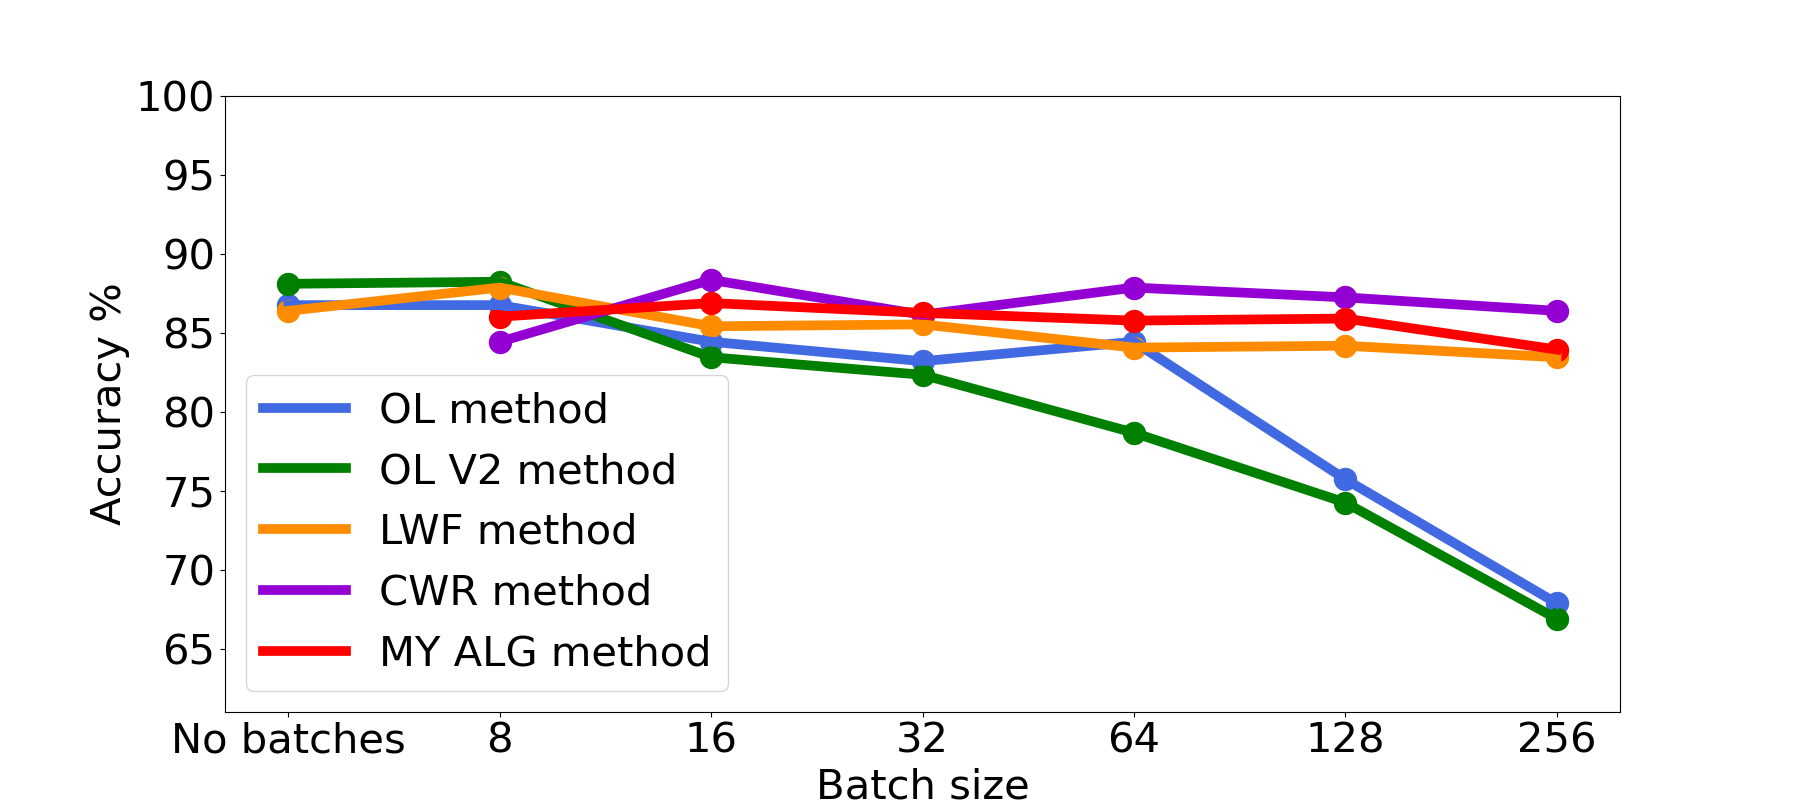
\includegraphics[width=100mm]{Figures/Chapter5/batch_size_letters.png} 
    \caption{PLACEHOLDER}
    \label{fig:batch_size_letter}    
\end{figure}
%

\chapter{Conclusion}






LA BIBLIOGRAFIA NON FUZNIONA
\printbibliography[heading=bibintoc]


\end{document}
